% !TeX program = lualatex

% Copyright (c) 2020-2025 Simon Crase

% Permission is hereby granted, free of charge, to any person obtaining a copy
% of this software and associated documentation files (the "Software"), to deal
% in the Software without restriction, including without limitation the rights
% to use, copy, modify, merge, publish, distribute, sublicense, and/or sell
% copies of the Software, and to permit persons to whom the Software is
% furnished to do so, subject to the following conditions:

% The above copyright notice and this permission notice shall be included in all
% copies or substantial portions of the Software.

% THE SOFTWARE IS PROVIDED "AS IS", WITHOUT WARRANTY OF ANY KIND, EXPRESS OR
% IMPLIED, INCLUDING BUT NOT LIMITED TO THE WARRANTIES OF MERCHANTABILITY,
% FITNESS FOR A PARTICULAR PURPOSE AND NONINFRINGEMENT. IN NO EVENT SHALL THE
% AUTHORS OR COPYRIGHT HOLDERS BE LIABLE FOR ANY CLAIM, DAMAGES OR OTHER
% LIABILITY, WHETHER IN AN ACTION OF CONTRACT, TORT OR OTHERWISE, ARISING FROM,
% OUT OF OR IN CONNECTION WITH THE SOFTWARE OR THE USE OR OTHER DEALINGS IN THE
% SOFTWARE.

\documentclass[]{article}
\usepackage{caption}
\usepackage{subcaption}
\usepackage{graphicx}
\usepackage{float}
\usepackage{url}
\usepackage{amsmath}
\usepackage{amssymb}
\usepackage{amsthm}
\usepackage{tocloft}
\usepackage{cancel}
\usepackage{thmtools}
\usepackage{gensymb}
\usepackage{braket}
\usepackage{tikz-feynman}
\usepackage{tikz}
\usepackage{pgfplots}
\usepackage{mathtools}
\usepackage{color}
\usepackage{colortbl}
\usepackage[toc,nonumberlist]{glossaries}
\usepackage{glossaries-extra}
\newcommand\numberthis{\addtocounter{equation}{1}\tag{\theequation}}
\newcommand{\Schr}{{Schr\"odinger }}
\newtheorem{thm}{Theorem}
\newtheorem{defn}[thm]{Definition}
\newtheorem{cor}[thm]{Corollary}
\newtheorem{lemma}[thm]{Lemma}
\graphicspath{{figs/}}
\widowpenalty10000
\clubpenalty10000
\setcounter{tocdepth}{2}

%opening
\title{Theoretical Minimum\\Particle Physics 1\\Basic Concepts}
\author{Simon Crase (compiler)\\simon@greenweaves.nz}
\makeglossaries
\loadglsentries{glossary-entries}
\begin{document}

\maketitle

\begin{abstract}
These are my notes for \emph{New Revolutions in Particle Physics 1}  from Leonard Susskind's \emph{Theoretical Minimum} series \cite[Particle Physics 1: Basic Concepts]{susskind2007theoretical}.

\begin{quotation}
	Revolutionary new concepts about elementary particles, space and time, and the structure of matter began to emerge in the mid-1970s. Theory got far ahead of experiment with radical new ideas such as grand unification and supersymmetry, but the concepts have never been experimentally tested. Now all that is about to change. The \glsdesc{gls:LHC}, or \gls{gls:LHC}, has finally been built and is about to confront theory with experiment. This course is devoted to these theoretical ideas and how they will be tested.
\end{quotation}

Disclaimer: I have created these notes as an aide-m\'emoire for my own use; if you find them useful, you are welcome, but I'd appreciate hearing from you. They are not intended as a substitute for listening to the lectures. The intellectual property for all material derived from the lectures belongs, of course, to Professor Susskind; any mistakes, however, are my own.

\end{abstract}

\tableofcontents
\listoffigures
\listoftables
\listoftheorems

\section{Particles and Light}

\subsection{Introduction}
This lecture contains  facts from other courses, which will be used in later lectures.

Particle physics is about the question: is matter discrete? If so we will call the smallest things "particles". If matter forms a continuum, we have fields.

Which is correct? Both and neither.

The first evidence for atoms came from chemistry. John Dalton found that the mass of one mole of each substance was an integer multiple of the mass of a mole of hydrogen; this suggested that there are building blocks. We now know that mass of molecule is mass of protons, electrons (very small), and neutrons, which have nearly the same mass as protons. 
 
Figure \ref{fig:em:wave} illustrates an electromagnetic wave. We need the concepts of wavelength, $\lambda$, and period, $T$.

We have
\begin{align*}
	\frac{\lambda}{T}=&c\\
	f=&\frac{1}{T} \text{, so}\\
	\lambda f =& c\text{. Physicists tend to measure frequency in radians per second:}\\
	\omega =& 2 \pi f \text{, so} \\
	\omega =& \frac{2 \pi c}{\lambda} \numberthis \label{eq:omega:lambda}
\end{align*}

\begin{figure}[H]
	\caption{An electromagnetic wave}\label{fig:em:wave}  
	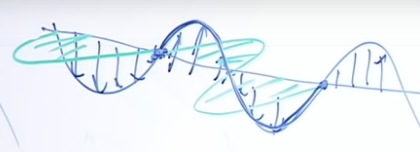
\includegraphics[width=0.9\textwidth]{Wavelength}
\end{figure}

\subsection{Wave/particle duality.}

A photon has energy:
\begin{align*}
	E=&\hslash \omega \text{. Energy of single photon.} \numberthis\label{eq:E_omega}\\
	E_{ray}=&n \hslash \omega \text{. Energy of ray.}
\end{align*}

(I learned quantum mechanics using Planck's constant, $h$, rather than Dirac's $\hbar$; $hf=\hbar\omega$.) 

In modern usage, mass is what used to be called rest mass. $E = m c^2$ only for stationary object.

In particle physics we choose units such that $c=1$ and $\hslash=1$. In this course, $c$ and $\hslash$ will appear explicitly only when Prof. Susskind wants to show the magnitude of some quantity.

Energy depends on the motion of the object as seen by the observer: it isn't a universal thing that everyone will agree on.

Light has energy and momentum (not mass): 

\begin{align*}
	\left|P\right|=&\frac{E}{c} \\
	=&\frac{\hslash \omega}{c} \text{, from (\ref{eq:E_omega})}\\
	=& \frac{2 \pi \hslash}{\lambda} \text{, from (\ref{eq:omega:lambda}). c.f. Harmonic Oscillator.}\numberthis\label{eq:P:lambda}
\end{align*}

This is why we need larger and larger instruments to observe smaller particles!
To see really small things, we need particles with high energy and momentum.


\section{Quantum field theory}

\subsection{Mathematical Preliminaries}

Consider a classical wave $A \sin(kx)$. Energy is proportional to $A^2$, but also to the number of photons, $n$: $E \propto n \hslash \omega$, $A \propto \sqrt{n}$.

Generally, equations containing $c$ apply for photons only. For non-relativistic particles:
\begin{align*}
	E=&\frac{p^2}{2m}\\
	f =& \frac{h}{2 m \lambda^2} \text{. c.f. \Schr equation!}
\end{align*}

\begin{itemize}
	\item Phase Velocity: velocity of wave packet;
	\item Group velocity: velocity of troughs and peaks--identified with particle velocity.
\end{itemize}

For light waves, phase and group velocities are the same, but this isn't true for most particles. Phase velocity can exceed $c$, but it can't transmit information--Section \ref{section:phase:group:velocities}.

Space is infinite. If physics is the art of getting problems into a shape that computers can solve, we need to remove infinities.

Let's look at 1 dimensional waves. In order to get rid of infinities, we can restrict to fixed length $L$: reflecting boundary condition at ends. But this violates conservation of momentum: when wave bounces momentum reverses. Instead use a topological ''circle''\footnote{I.e. we just assume that the ends are connected} circumference $L$--periodic boundary conditions. This gets rid of infinity and preserves conservation of momentum at a cost: momentum is quantized: 

\begin{align*}
	\lambda =& \frac{L}{N} \text{ for some integer $N$}\\
	P =& \frac{h}{\lambda} \text{ allowable momenta}\\
	=& \frac{h N}{L} \numberthis \label{eq:momenta:finit:volume}
\end{align*}

Now make into a real circle, radius $R$, and redefine $L=PR$ to be \emph{angular momentum}.

\begin{align*}
	P =& \frac{h N}{2 \pi R}\\
	L =& N \frac{h}{2 \pi}\\
	=& N \hslash \text{ independent of $R$.}
\end{align*}

\subsection{Quantum field theory}

Start with harmonic oscillator: a wave is a collection of harmonic oscillators. Energy is quantized: 0, $\hslash \omega$, $2\hslash \omega$...

Introduce operators:

\begin{align*}
	a^+ \ket{n} =& \sqrt{n+1} \ket{n+1} \text{, creation operator} \numberthis \label{eq:creation}\\
	a^- \ket{n} =& \sqrt{n} \ket{n-1} \text{, annihilation operator} \numberthis \label{eq:annihilation} \\
	a^+ a^- \ket{n} =& n \ket{n} \text{, or}\\
	a^+ a^-  =& n \text{. Similarly}\\
	a^- a^+  =& n+1\\
	[a^-, a^+] =& 1
\end{align*}

Return to world on a circle--$\omega_N$--equivalent to oscillator. State is $\ket{n_1,n_2, n_3,...}$--occupation numbers. 
\begin{defn}[quantum field]
	A quantum field is a collection of harmonic oscillators, together with annihilation operators and creation operators.
\end{defn}

\section{Quantum fields and particles}

\begin{align*}
	\text{Wave} =& e^{i k x} \text{, $k$ is wave number}\\
	P=&\hslash k\\
	n(k) =& \text{ occupation number.}
\end{align*}

We represent the state of a 1D circular system by occupation numbers, $\ket{...n(-1), n(0), n(1), n(2)...}$, and introduce operators $a^+(k)$, $a^-(k)$. 
\begin{align*}
a^+(1)\ket{...n(-1), n(0), \underbrace{n(1)}_\text{target of $a^+(1)$}, n(2)...}=& \sqrt{n(1)+1}\ket{...n(-1), n(0), n(1)+1, n(2)...}
\end{align*}
$a^+(k)$, $a^-(k)$ are quantum mechanical versions of the Fourier coefficients of a field $\Psi$.

Here is a classical wave:
\begin{align*}
	\Psi(x) =& \sum_k \alpha(k) e^{ikx}\\
	\Psi^*(x) =& \sum_k \alpha^*(k) e^{-ikx}
\end{align*}

We quantize as shown in (\ref{eq:q:1}) and (\ref{eq:q:2}) to produce a quantum field:
\begin{align*}
	\alpha(k) \rightarrow& a^-(k) \numberthis \label{eq:q:1}\\
	\alpha^*(k) \rightarrow& a^+(k) \numberthis \label{eq:q:2}\\
	\Psi(x) =& \sum_k a^-(k) e^{ikx} \numberthis \label{eq:Psi}\\
	\Psi^\dagger(x) =& \sum_k a^+(k) e^{-ikx} \numberthis \label{eq:Psi:dagger}
\end{align*}

We need to justify (\ref{eq:q:1}) and (\ref{eq:q:2}) in some appropriate limit.

How can we describe scattering? Imagine scattering so a particle with momentum $k_7$ becomes a particle with momentum $k_9$: $a^+(k_9)a^-(k_7)\ket{0,0,..1,0,0}$.

What if laws of physics allows number of particles to change? $a^+(k_{16})a^+(k_9)a^-(k_7)\ket{0,0,..1,0,0}$. We can't do this in regular quantum mechanics.

What does $\Psi^\dagger$ do? Start with the vacuum $\ket{0}$.

\begin{align*}
	\Psi^\dagger(x)\ket{0} =& \sum_k a^+(k) e^{-ikx} \ket{0} \text{ from (\ref{eq:Psi:dagger})}\\
	=& \sum_k e^{-ikx} \underbrace{a^+(k) \ket{0}}_\text{One particle state with momentum $k$} \\
	=& \sum_k e^{-ikx} \ket{k} \text{. Superposition gives particle at definite position.}
\end{align*}

If we make the circle larger and larger, $\sum \rightarrow \int$.

What does $\Psi$ do? It annihilates a particle at $x$.

Locality: when something happens, it happens at one spot. Figure \ref{fig:ex:locality} is an example of one particle being replaced by two.

\begin{figure}[H]
	\caption[Example of locality: one particle is replaced by two]{Example of locality: $\Psi^\dagger(x)\Psi^\dagger(x)\Psi(x)\ket{...}$}\label{fig:ex:locality}
	\begin{center}
		\feynmandiagram [horizontal=i1 to a] {
			i1[] -- [fermion,momentum'=\(k\)] a[particle=\(x^{\prime}\)],
			a --[fermion] f1[],
			a--[fermion] f2[],
		};
	\end{center}
\end{figure}



Start with state $\ket{0,...\underbrace{1}_\text{$k_i$},0,000}$.

We assume that $k_i$ denotes the index of the only momentum with a non-zero index.
\begin{align*}
\Psi^\dagger(x)\Psi^\dagger(x)\Psi(x)\ket{0,...1,0,000}=&\sum_m a^+(m) e^{-imx} \sum_l a^+(l) e^{-ilx} \sum_k a^-(k) e^{ikx} \ket{...}\\
=&\sum_m a^+(m) e^{-imx} \sum_l a^+(l) e^{-ilx} a^-(k_i) e^{ik_ix} \ket{...}\\
=&\sum_m a^+(m) e^{-imx} \sum_l a^+(l) e^{-ilx}  e^{ik_ix} \ket{0}\\
=&\sum_{l,m}  e^{-imx}  e^{-ilx}  e^{ik_ix} \underbrace{\ket{001001...}}_\text{$l$ and $m$ are indices of $1s$.}\\
\triangleq &\sum_{l,m}   e^{i(k-l-m)x} \ket{l,m}
\end{align*}

This isn't true if $l=m$! We have two application of $a^+(m)$, so vacuum becomes $\sqrt{2}\ket{...2...}$. Probability of two particles coming out in same state is twice probability of them being in different states.

For the time being we ignore conservation laws!

Consider generating photon at a position where there is a pre-existing photon with momentum $l$--Figure \ref{fig:simple:decay}.
\begin{figure}[H]
	\begin{center}
		\caption[Generating photon  where there is a pre-existing photon]{Generating photon at a position where there is a pre-existing photon with momentum $l$.}\label{fig:simple:decay}
		\feynmandiagram[layered layout,horizontal=in1 to out1]{
			in1--[photon]c--[photon,edge label=\(l\)]out1,
			c--[photon]out2,
		};
	\end{center}
\end{figure}

\begin{align*}
\Psi(x)^\dagger\ket{l} =& \sum_k a^+(k) e^{-ikx} \ket{l}\\
=& \sum_{k\ne l} e^{-ikx} \ket{k,l} + \sqrt{2} e^{-ilx} \ket{l,l}
\end{align*}

Stimulated emission: higher probability of generating particles that are already there (c.f. spontaneous emission). This is true for Bosons, but not Fermions.
 
 Laws for Bosons
 \begin{align*}
 [a^+(k),a^+(l)] =& 0\\
 [a^-(k),a^-(l)] =& 0\\
 [a^-(k),a^+(l)] =& \delta_{k,l}\\
 \Psi(x) =& \sum_k a^-(k) e^{ikx} \\
 \Psi^\dagger(x) =& \sum_k a^+(k) e^{-ikx}
 \end{align*}
 
 \begin{align*}
 \frac{1}{L}\int_\frac{-L}{2}^\frac{L}{2} dx \Psi^\dagger(x) \Psi(x) =& \frac{1}{L} \int_\frac{-L}{2}^\frac{L}{2} dx \sum_k a^+(k) e^{-ikx} \sum_l a^-(l) e^{ilx}\\
 =& \sum_k a^+(k) \sum_l a^-(l) \frac{1}{L} \int_\frac{-L}{2}^\frac{L}{2} e^{-ikx} e^{ilx} dx\\
 =& \sum_k a^+(k) \sum_l a^-(l) \frac{1}{L} \int_\frac{-L}{2}^\frac{L}{2} e^{-i(k-l)x} dx\\
  =& \sum_k a^+(k) \sum_l a^-(l) \delta_{k,l}\\
 =&  \sum_k \underbrace{a^+(k) a^-(k)}_\text{Occupation number}\\
 =& N \text{, total number of particles.}\\
 \Psi^\dagger(x) \Psi(x) =& \text{ density of particles at $x$}.
 \end{align*}


\section{More quantum field theory}

\subsection{Mathematical Preliminaries}

\subsubsection{Dirac Delta function}

\begin{align*}
	\text{For } k =& \frac{2 \pi n}{L}\\
	\int_{-\frac{L}{2}}^{\frac{L}{2}} e^{ikx} dx =& L \text{, if $k =0$}\\
	=& 0 \text{, otherwise}\\
	\rightarrow& 2 \pi \delta(k) \text{ as $k \rightarrow \infty$}
\end{align*}

We will use \emph{ket} vectors for initial states, \emph{bra} for final. This will help with bookkeeping.

\subsubsection{Creation and annihilation operators operating on bra vectors}

\begin{align*}
	\braket{n|m} =& \delta_{n,m}\numberthis \label{eq:orthogonal} \text{. We want the following}\\
	\braket{n|(a^+|m)} =& \braket{(n|a^+)|m}  \numberthis \label{eq:consistency}\\
	=& \sqrt{m+1} \braket{n|m+1} \text{, from (\ref{eq:creation})}\\
	=& \sqrt{m+1} \delta_{n,m+1} \text{, from (\ref{eq:orthogonal})} \text{, so we define}\\
	\bra{n} a^+ \triangleq & \sqrt{n} \bra{n-1} \text{ to satisfy (\ref{eq:consistency}), and} \numberthis \label{eq:bra:create}\\
	\bra{n} a^= \triangleq & \sqrt{n+1} \bra{n-1} \numberthis \label{eq:bra:annihilate}
\end{align*}
Example: calculate an expression two different ways.
\begin{align*}
	\braket{n|(a^+a^-|n)} =& \sqrt{n}\braket{n|(a^+|n-1)}\\
	=& (\sqrt{n})^2 \braket{n|n} \text{ from (\ref{eq:bra:create})}\\
	=& n\\
	\braket{(n|a^+a^-)|n} =& \sqrt{n} \braket{(n-1|a^-)|n}\\
	=& n \braket{n|n} \text{ from (\ref{eq:bra:annihilate})}
\end{align*}

\subsection{Quantum Fields}

The only way we can study particles is to collide them; quantum field theory is the mathematical tool.

We will set $\hslash=1$, so $P=k$, and we will take $X$ and $P$ to be 3 dimensional.
\begin{align*}
\Psi^\dagger(X)(X,t) \triangleq& \sum_k a^+(k) e^{-ikX} e^{i \omega(k) t} \\
\Psi(X)(X,t) \triangleq& \sum_k a^-(k) e^{ikX} e^{- i \omega(k) t}
\end{align*}

\begin{align*}
\omega =& E \text{ and}\\
E =& \frac{P^2}{2m} \text{, whence}\\
\omega =& \frac{k^2}{2m} \numberthis \label{eq:omega:k}
\end{align*}
We  determine the differential equation satisfied by $\Psi^\dagger(X)$.

\begin{align*}
\dot{\Psi^\dagger(X)} =&  \sum_k i \omega(k) a^+(k) e^{-ikX} e^{i \omega(k) t}\\
\frac{\partial^2 \Psi^\dagger(X)}{\partial X^2} =& \sum_k -k^2 a^+(k) e^{-ikX} e^{i \omega(k) t} \numberthis \label{eq:omega:dot}\\
 =& - \sum_k 2m \omega a^+(k) e^{-ikX} e^{i \omega(k) t} \text{ from (\ref{eq:omega:k})}\\
 \frac{1}{2m} \frac{\partial^2 \Psi^\dagger(X)}{\partial X^2} =& - \sum_k \omega a^+(k) e^{-ikX} e^{i \omega(k) t}\\
 =& -\frac{1}{i} \frac{\Psi^\dagger(X)}{\partial t}\\
  i \frac{\Psi^\dagger(X)}{\partial t} =&  \frac{1}{2m} \frac{\partial^2 \Psi^\dagger(X)}{\partial X^2} \text{ From (\ref{eq:omega:dot}). This is \Schr's equation for field!}
\end{align*}

Consider particle scattering from heavy target; we show it conserves energy, but not momentum--Figure \ref{fig:particle:heavy:target}. Assume scattering probability independent of time.

\begin{figure}[H]
	\caption{Particle being absorbed and then re-emitted}\label{fig:particle:heavy:target}
	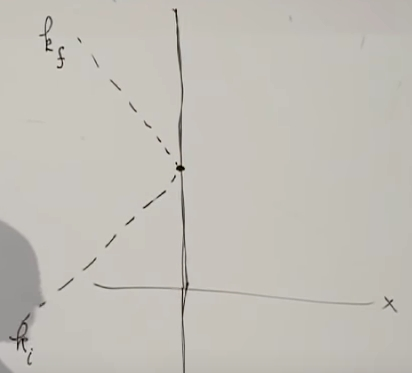
\includegraphics[width=0.8\textwidth]{particle-heavy-target}
\end{figure}

We want the probability of emitting one particle in final state (Introduce coupling constant $g$)--$\big| \bra{k_f} g \int dt \Psi^\dagger(0,t)\Psi(0,t)\ket{k_i} \big|^2$

\begin{align*}
	&\bra{k_f} g \int dt \sum_l \underbrace{a^+(l) e^{i \omega_l t}}_\text{contributes iff $l==k_f$} \sum_k \underbrace{a^-(k) e^{-i \omega_k t} \ket{k_i}}_\text{contributes iff $k==k_i$}\\
	=&\bra{k_f} g \int dt a^+(k_f) e^{i \omega_{k_f} t}  a^-(k_i) e^{-i \omega_{k_i} t} \ket{k_i}\\
	=& g \int dt e^{i(\omega_{k_f}-\omega_{k_i})}\cancel{<0|0>}\\
	=& 2 \pi g \delta(\omega_{k_f}-\omega_{k_i}) \text{--conservation of energy.} \numberthis \label{eq:conservation:energy}
\end{align*}

Conservation of energy works only because of time symmetry!

Probability $\propto g^2$.

Prof. Susskind has shown:
\begin{itemize}
	\item Definition of coupling constant;
	\item Integration over time is the thing that ensures energy conservation;
	\item Scattering amplitude.
\end{itemize}

NB.\begin{itemize}
	\item  If X not zero (say $X_s$), then amplitude gets a phase of $e^{i(k_f-k_i)S_s}$, which doesn't affect probability.
	\item if $g$ is a function of time, it generally means that we are ignoring something.
\end{itemize}

To reiterate: $\Psi$ and $\Psi^\dagger$ are the tools that let us discuss particle interactions.

What if we are dealing with an electron? Each particle has its own $\Psi$. What if one electron goes in but two come out-- $\Psi^\dagger(0,t)\Psi^\dagger(0,t)\Psi(0,t)$? Or two in, two out--$\Psi^\dagger(0,t)\Psi^\dagger(0,t)\Psi(0,t)\Psi(0,t)$? Which are allowed? One rule is that there must be the same number of $\Psi^\dagger$s and $\Psi$s. Imagine multiplying by a phase:

\begin{align*}
\Psi \rightarrow & e^{i\alpha} \Psi \numberthis \label{eq:conservation:charge1}\\
\Psi^\dagger \rightarrow & e^{-i\alpha} \Psi^\dagger \numberthis \label{eq:conservation:charge2}
\end{align*}

Allowable combinations are invariant under multiplication by $e^{i\alpha}$--charge is conserved. Table \ref{table:conserve} shows some pairs of symmetries and conservation laws.

\begin{table}[H]
	\caption{Invariance and Conservation Laws}\label{table:conserve}
	\begin{center}
			\begin{tabular}{|l|l|l|}  \hline
				Invariance&Conservation&Ref\\ \hline
				Time& Energy&(\ref{eq:conservation:energy})\\  \hline
				Space&Charge&(\ref{eq:conservation:charge1}),  (\ref{eq:conservation:charge2})\\ \hline
				Phase&Momentum&Section \ref{sec:momentum:conservation}\\ \hline
			\end{tabular}
	\end{center}
\end{table}

NB, this isn't a real electron, as $\Psi$ is for Bosons. A negative pion would be OK.


\section{Energy conservation and waves}\label{sec:energy:conservation}

\subsection{Phase Velocity and Group Velocity}\label{section:phase:group:velocities}

\subsubsection{Phase Velocity and Group Velocity of non-relativistic particles}
Generally phase velocity doesn't have anything to do with measurable things in quantum mechanics. Group velocity is what counts.

Consider $\sin(kx-\omega t)$. The wave moves so that $kx-\omega t$ remains constant.
\begin{align*}
	x =& \underbrace{\frac{\omega}{k}}_{\mathclap{\substack{\text{phase }\\
															\text{velocity}}}} t\\
	\omega =& \frac{2 \pi}{T}\\
	k =& \frac{2 \pi}{\lambda}
\end{align*}

This is connected with the \Schr equation, since $\omega$ is energy, and $k$ momentum, so:
\begin{align*}
	\omega=&\frac{k^2}{2m} \text{, whence} \numberthis \label{fig:phase:c}\\
	\frac{\omega}{k}=&\frac{k}{2m} \text{, phase velocity.}\\
	=& \frac{v}{2}  \text{, where $v$ is velocity of classical particle.}
\end{align*}
 Let's add a constant to frequency, hence to the energy:
\begin{align*}
	\omega=&\frac{k^2}{2m}+c 
\end{align*}
Adding $c$ changes the phase velocity--but changing $E$ by an additive constant has no physical effect! Now we write:
\begin{align*}
	\Psi =& \sum_k a^-(k) e^{ikx}e^{- i \omega(k) t} e^{-i c t}
\end{align*}
Given a solution to the \Schr equation, adding a constant to the phase just multiplies $\Psi$ by $e^{-i c t}$. All of the quantities of physical interest that are made out of the \Schr field involve $\Psi\Psi^\dagger=\cancel{e^{-i c t}}\Psi \cancel{e^{+i c t}}\Psi^\dagger$: e.g. probability density, expectation values. There is no physical sense to adding a constant, but it does change the phase velocity. We see that the phase velocity isn't measurable; it is an artifact of the mathematics. On the other hand, the group velocity does mean something.

Given a bunch of plain waves, how can we get them to add up to a concentrated lump? (Which will turn out to move with something called the group velocity.) The answer is destructive interference: the waves add someplace, and cancel out in other places. If we have a bunch of waves, and are interested in how the waves of slightly different frequency reinforce each other, let's look at two waves, whose momenta are close, and try to see how it all works. We will try to follow where the constructive interference takes place between two waves.

\begin{align*}
	\sin(kx-\omega(k)t) +& \sin(k^\prime x-\omega(k^\prime)t)\text{ will reinforce each other when}\\
	kx-\omega(k)t=&k^\prime x-\omega(k^\prime)t\text{, i.e. when}\\
	x =& \frac{\omega-\omega^\prime}{k-k^\prime}t\\
	\rightarrow & \underbrace{\frac{d \omega}{dk}}_{\mathclap{\substack{\text{group  }\\
	\text{velocity}}}} t \text{, as $k-k^\prime \rightarrow 0$}
\end{align*}
The point where the waves reinforce each other will travel with the \emph{group velocity}:
\begin{align*}
	V_g\triangleq&\frac{d \omega}{dk}\\
	=&\frac{k}{m} \text{, from \eqref{fig:phase:c}}
\end{align*}
\begin{itemize}
	\item The group velocity does not depend on $c$
	\item The group velocity matches the velocity of a non-relativistic particle.
\end{itemize}

\subsubsection{Phase Velocity and Group Velocity of Relativistic Particles}

We will calculate the phase velocity and group velocity  of a relativistic particle, starting with the relationship between energy and momentum. 

\begin{align*}
	E =& \sqrt{P^2 + m^2} \text{, which leads to the wave equation}\\
	\omega =& \sqrt{k^2 + m^2}
\end{align*}
At speed of light(m=0), so
\begin{align*}
	\omega =& \left| k \right|\\
	V_p =& \frac{\omega}{k} \text{ phase velocity of photon waves}\\
	 =&1\\
	 V_g =& \frac{d\omega}{dk} \text{ group velocity of photon waves}\\
	 =&1
\end{align*}
So the group velocity and phase velocity are the same for a massless particle. Now lets us make $m>0$
\begin{align*}
	V_p =& \frac{\omega}{k}\\
	=&\sqrt{\frac{k^2+m^2}{k^2}}\\
	=&\sqrt{1+\frac{m^2}{k^2}} \numberthis \label{eq:rel:phase:V}\\
	>&1
\end{align*}
\begin{align*}
	V_g =& \frac{d\omega}{dk} \\
	=& \frac{\cancel{2}k}{\cancel{2}\sqrt{k^2+m^2}}\\
	=& \frac{1}{\sqrt{1+\frac{m^2}{k^2}}} \numberthis \label{eq:rel:group:V}\\
	<&1 \text{. Combining \eqref{eq:rel:phase:V} and \eqref{eq:rel:group:V}}\\
	V_p V_g =& 1
\end{align*}

If $\omega\propto k$, the waves all have the same phase and group velocities irregardless of frequency: the difference between group and phase velocities is connected to dispersion.

\subsection{Momentum Conservation}\label{sec:momentum:conservation}

In the discussion around Figure \ref{fig:particle:heavy:target}, leading to \eqref{eq:conservation:energy}, we saw how time invariance led to the conservation of energy. We integrated over all possible times; because the process could happen at any time:
\begin{align*}
	&\bra{k_f}  \int dt a^+(k_f) e^{i \omega_{k_f} t}  a^-(k_i) e^{-i \omega_{k_i} t} \ket{k_i}\\
	=&  \int dt e^{i(\omega_{k_f}-\omega_{k_i})}\cancel{<0|0>}\\
	=& 2 \pi  \delta(\omega_{k_f}-\omega_{k_i})
\end{align*}
Now we will show how a process that can occur anywhere in space leads to conservation of momentum.  Figure \ref{fig:split:particle} shows a particle splitting into two particles. 
 
\begin{figure}[H]
	\begin{center}
		\caption[Split Particle at any position $x$]{Split Particle at any position $x$. A particles is eaten at $x$, and two particles are created at the same point: $\bra{k_1^\prime,k_2^\prime}\int \Psi^\dagger(x)\Psi^\dagger(x)\.\Psi(x) dx\ket{k}$}\label{fig:split:particle}
		\feynmandiagram[horizontal'=out1 to out2]{
			in1--[fermion, edge label=\(k\)]c--[fermion, edge label=\(k_1\)]out1,
			c--[fermion, edge label=\(k_2\)]out2,
		};
	\end{center}
\end{figure}

\begin{align*}
	\bra{k_1^\prime,k_2^\prime}&\int \Psi^\dagger(x)\Psi^\dagger(x)\Psi(x) dx\ket{k}\\
	=&\bra{k_1^\prime,k_2^\prime}\int \underbrace{a^+(k_1^\prime) a^+(k_2^\prime)}_{\mathclap{\substack{\text{Create 2}\\
		\text{particles}}}} \underbrace{a^-(k)}_\text{Eat particle} \underbrace{e^{ikx} e^{-i(k_1^\prime+k_2^\prime)x}}_{\mathclap{\substack{\text{integrates to }\\
	\text{Dirac-$\delta$--(\ref{eq:conservation:energy})}}}} dx\ket{k}
\end{align*}

So invariance under space translation yields conservation of momentum.

Another \emph{possible} symmetry: $\Psi \rightarrow e^{i \lambda} \Psi$. There is no change to probabilities if number of $\Psi$s is same as number of $\Psi^\dagger$s. This is connected with conservation of charge.

\subsection{Fermions}

\subsubsection{Introduction to Fermions}

\begin{itemize}
	\item Can have any number of Bosons in any state (same place);
	\item Bosons have a tendency to accumulate in the same state. E.g. consider a particle that decays and emits a photon. If lots of other photons already on some state, decay will preferentially favour that state.
\end{itemize}

Fermions cannot be in same state (Pauli Exclusion Principle). We will start the same way we did with Bosons.

\begin{align*}
	\Psi(x) =& \sum_k a^-(k) e^{ikx}
\end{align*}
The state of the system is once again a vector showing the number of particles in each state, but these numbers can be $0$ or $1$ only because of the Pauli exclusion principle: $\ket{001...01010...}$. Again we have:
\begin{align*}
	\Psi^\dagger(x) =& \sum_k a^+(k) e^{-ikx}
\end{align*}

Focus on one state, either full $(\ket{1})$ or empty $(\ket{0})$: those are only two possibilities. What are the algebraic rules for creation and annihilation operators?

\begin{align*}
	c^+\ket{0} =& \ket{1} \text{, for Fermions use $c$ rather than $a$}\\
	c^+\ket{1} =& 0 \text{, i.e. $\psi(x) \equiv 0$}\\
	c^-\ket{1} =& \ket{0}\\
	c^-\ket{0} =& 0\\
\end{align*}

We deduce:
\begin{align*}
	c^+c^-\ket{0} =& 0\\
	c^-c^+\ket{0} =& \ket{0}\\
	(c^+c^-+c^-c^+)\ket{0} =& \ket{0}\\
	c^+c^-\ket{1} =& \ket{1} \\
	c^-c^+\ket{1} =&0 \\
	(c^+c^-+c^-c^+)\ket{1} =& \ket{1}
\end{align*}
We define the anticommutator:
\begin{align*}
	\{c^+,c^-\} \triangleq& (c^+c^-+c^-c^+) \text{, then}\\
	\{c^+,c^-\} =& 1\\
	\{c^+,c^+\} =&0 \\
	\{c^-,c^-\} =&0
\end{align*}
So Fermions have parallel mathematics to Bosons: $[,] \leftrightarrow \{,\}$. We cannot put two particles into the same state, as $c^+c^+=0$.

What about different momenta? We can show that:
\begin{align*}
	\{c^+_k,c^-_{k^\prime} \} =& \delta_{k,k^\prime} \\
	\{c^+_k,c^+_{k^\prime} \} =&0 \\
	\{c^-_k,c^-_{k^\prime} \} =&0
\end{align*}

This shows we can't put two Fermions into the same momentum state. Can we have two Fermions at the same position? Let's try to create them at the origin.

\begin{align*}
	\Psi^\dagger(0) \Psi^\dagger(0) \ket{0} =& \sum_{k,k^\prime} c^+_k c^+_{k^\prime} \ket{0}\\
	==& \frac{1}{2} \sum_{k,k^\prime} \{c^+_k, c^+_{k^\prime}\} \ket{0}\\
	=& 0
\end{align*}

So the answer is no: we can't have two Fermions in the same quantum state (e.g. momentum and spin). So we can't have an electron laser.

There was a question about whether two electrons in two different hydrogen atoms can have the same momentum. LS explained that the electrons are in energy states (not momentum), and each has a separate wave function. They are distinguishable by position.

A system is a collection of degrees of freedom. In classical mechanics, a state is a a set of values for the degrees of freedom; in \glsdesc{gls:QM} a state is everything you have to specify to encompass everything that can be measured.

\subsubsection{Ground State}
We now compare the ground state of a system of Bosons with the ground state of a system of Fermions. In Figure \ref{fig:electons:confined:momentum} we have some particles confined in momentum space. If particles are confined to be within a given volume, then momenta are discrete--\eqref{eq:momenta:finit:volume}. The same thing happens if the momenta are confined.

\begin{figure}[H]
	\begin{center}
		\caption[Particles confined in momentum space]{Allowable momenta of particles confined in periodic 3 dimensional box in momentum space}\label{fig:electons:confined:momentum}
		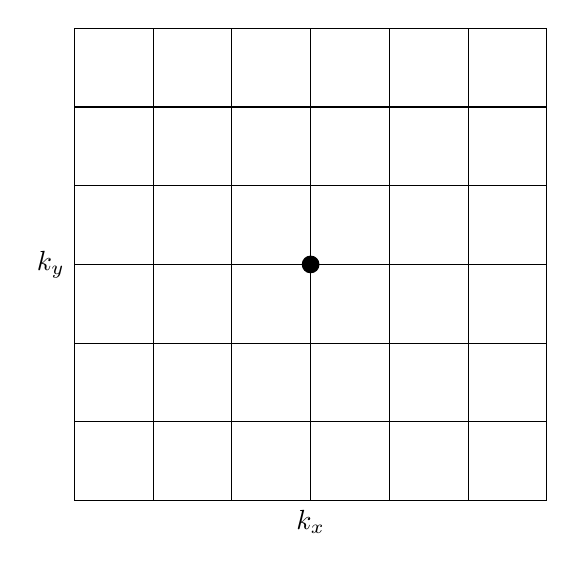
\begin{tikzpicture}
			\draw(0,0)--(0,6)--(6,6)--(6,0)--(0,0);
			\draw(1,0)--(1,6);
			\draw(2,0)--(2,6);
			\draw(3,0)--(3,6);
			\draw(4,0)--(4,6);
			\draw(5,0)--(5,6);
			\draw (6,1)--(0,1);
			\draw (6,2)--(0,2);
			\draw (6,3)--(0,3);
			\draw (6,4)--(0,4);
			\draw (6,5)--(0,5);
			\filldraw[black] (3,3) circle (3pt);
			\node[anchor=east] at (0,3) {$k_y$};
			\node[anchor=north] at (3,0) {$k_x$};
		\end{tikzpicture}
	\end{center}
\end{figure}

Let us take $N$ bosons, and put them into our box. Start with an empty box, and put one boson in. It will go to the state with lowest energy, zero momentum: $\frac{p^2}{m}=0$. Add another boson, in the same place, then another. We can put all $N$ bosons into the same momentum state, giving a \gls{gls:bose:conensate}. The wave function fills the box, and is uncertain about position.


This is very different from what happens with Fermions. Let us try adding Fermions, ignoring spin, each one going into the lowest energy state. We can add the first one in the zero momentum state, as in Figure \ref{fig:electons:confined:momentum}. Once we have filled that state, the next Fermion has to go into the next higher energy level--Figure \ref{fig:electons:lowest:energy}. We can continue, but after 5 electrons have been added (2 dimensional case, 7 for 3 dimensional) the level will be full--Figure \ref{fig:electons:lowest:energy:filled}. Continuing, we want to add electrons to the smallest sphere hat we can--Figure \ref{fig:electons:crowd:into:sphere}. This will have a lot more energy than the corresponding Boson system. Moreover, the electrons will fill a sphere in momentum space, whose boundary depends on the number of electrons--the \gls{gls:fermi:sphere}. 

\begin{figure}[H]
	\caption{Adding more Fermions}\label{fig:adding:more:fermions}
	\begin{subfigure}{0.32\textwidth}
		\caption{Two electrons, lowest possible energy}\label{fig:electons:lowest:energy}
		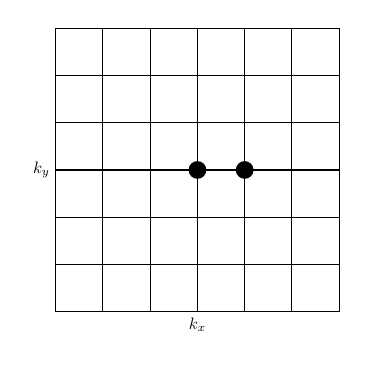
\begin{tikzpicture}[scale=0.6, transform shape]
			\draw(0,0)--(0,6)--(6,6)--(6,0)--(0,0);
			\draw(1,0)--(1,6);
			\draw(2,0)--(2,6);
			\draw(3,0)--(3,6);
			\draw(4,0)--(4,6);
			\draw(5,0)--(5,6);
			\draw (6,1)--(0,1);
			\draw (6,2)--(0,2);
			\draw (6,3)--(0,3);
			\draw (6,4)--(0,4);
			\draw (6,5)--(0,5);
			\filldraw[black] (3,3) circle (5pt);
			\filldraw[black] (4,3) circle (5pt);
			\node[anchor=east] at (0,3) {$k_y$};
			\node[anchor=north] at (3,0) {$k_x$};
		\end{tikzpicture}
	\end{subfigure}
	\hfill
	\begin{subfigure}{0.32\textwidth}
		\caption{Filled lowest two energy levels. The arrow indicates where a particle might go in the third energy level.}\label{fig:electons:lowest:energy:filled}
		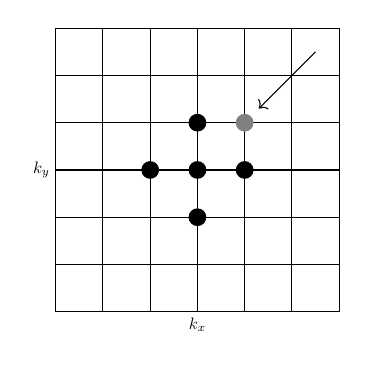
\begin{tikzpicture}[scale=0.6, transform shape]
			\draw(0,0)--(0,6)--(6,6)--(6,0)--(0,0);
			\draw(1,0)--(1,6);
			\draw(2,0)--(2,6);
			\draw(3,0)--(3,6);
			\draw(4,0)--(4,6);
			\draw(5,0)--(5,6);
			\draw (6,1)--(0,1);
			\draw (6,2)--(0,2);
			\draw (6,3)--(0,3);
			\draw (6,4)--(0,4);
			\draw (6,5)--(0,5);
			\filldraw[black] (3,3) circle (5pt);
			\filldraw[black] (4,3) circle (5pt);
			\filldraw[black] (2,3) circle (5pt);
			\filldraw[black] (3,2) circle (5pt);
			\filldraw[black] (3,4) circle (5pt);
			\filldraw[gray] (4,4) circle (5pt);
			\draw[->] (5.5,5.5)--(4.3,4.3);
			\node[anchor=east] at (0,3) {$k_y$};
			\node[anchor=north] at (3,0) {$k_x$};
		\end{tikzpicture}
	\end{subfigure}
	\hfill
	\begin{subfigure}{0.32\textwidth}
		\caption{$E=\frac{k^2}{2m}$, so there are more positions in each energy level as energy increases.}\label{fig:electons:crowd:into:sphere}
		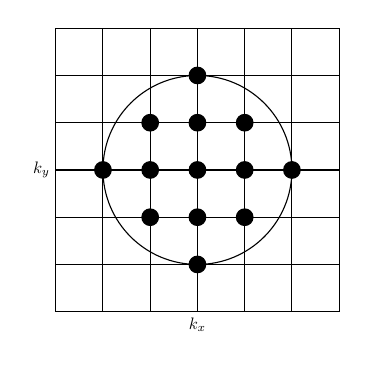
\begin{tikzpicture}[scale=0.6, transform shape]
			\draw(0,0)--(0,6)--(6,6)--(6,0)--(0,0);
			\draw(1,0)--(1,6);
			\draw(2,0)--(2,6);
			\draw(3,0)--(3,6);
			\draw(4,0)--(4,6);
			\draw(5,0)--(5,6);
			\draw (6,1)--(0,1);
			\draw (6,2)--(0,2);
			\draw (6,3)--(0,3);
			\draw (6,4)--(0,4);
			\draw (6,5)--(0,5);
			\filldraw[black] (3,3) circle (5pt);
			\filldraw[black] (4,3) circle (5pt);
			\filldraw[black] (2,3) circle (5pt);
			\filldraw[black] (3,2) circle (5pt);
			\filldraw[black] (3,4) circle (5pt);
			\filldraw[black] (5,3) circle (5pt);
			\filldraw[black] (1,3) circle (5pt);
			\filldraw[black] (3,1) circle (5pt);
			\filldraw[black] (3,5) circle (5pt);
			\filldraw[black] (4,4) circle (5pt);
			\filldraw[black] (2,2) circle (5pt);
			\filldraw[black] (2,4) circle (5pt);
			\filldraw[black] (4,2) circle (5pt);
			\draw(3,3) circle(2.0);
			\node[anchor=east] at (0,3) {$k_y$};
			\node[anchor=north] at (3,0) {$k_x$};
		\end{tikzpicture}
	\end{subfigure}
\end{figure}

We can move Bosons and Fermions out of the ground state, as shown in Figures \ref{fig:bosons:move:ground:state} and \ref{fig:fermions:move:ground:state}.
\begin{figure}[H]
	\caption[Moving Bosons and Fermions from lowest state]{Moving Bosons and Fermions from lowest state. We can think of  (\subref{fig:fermions:move:ground:state}) and (\subref{fig:fermi:surface}) as a low energy photon being absorbed by an electron,knocking it out and leaving a hole, or a photon annihilating to create an electron and a hole. }
	\begin{subfigure}[t]{0.45\textwidth}
		\caption{Initially the Bosons are all in the Ground State. Then we move one up to the first excited state. Which one? It doesn't matter for Bosons.}\label{fig:bosons:move:ground:state}
		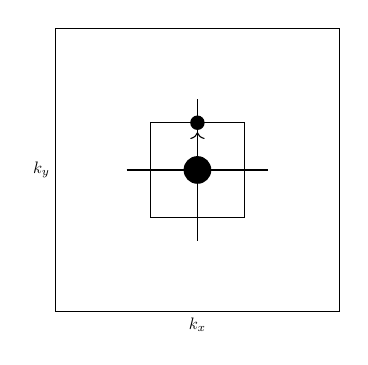
\begin{tikzpicture}[scale=0.6, transform shape]
			\draw(0,0)--(0,6)--(6,6)--(6,0)--(0,0);
			\draw(1.5,3)--(4.5,3);
			\draw(3,1.5)--(3,4.5);
			\draw(4,2)--(2,2)--(2,4)--(4,4)--(4,2);
			\filldraw[black] (3,4) circle (4pt);
			\filldraw[black] (3,3) circle (8pt);
			\draw[->](3,3)--(3,3.8);
			\node[anchor=east] at (0,3) {$k_y$};
			\node[anchor=north] at (3,0) {$k_x$};
		\end{tikzpicture}
	\end{subfigure}
	\hfill
	\begin{subfigure}[t]{0.45\textwidth}
		\caption{Moving Fermions to an excited state. It would not be a good idea to move an electron from deep inside the \gls{gls:fermi:sphere} as it would requires a lot of energy. (We can't move it within \gls{gls:fermi:sphere}, as we are dealing with Fermions.)}\label{fig:fermions:move:ground:state}
		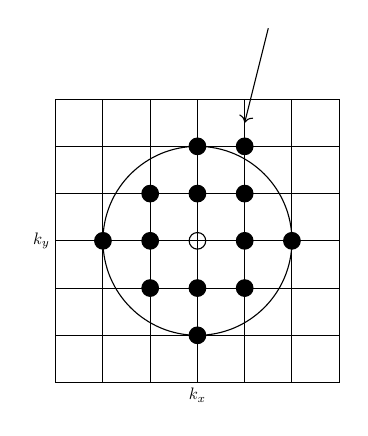
\begin{tikzpicture}[scale=0.6, transform shape]
			\draw(0,0)--(0,6)--(6,6)--(6,0)--(0,0);
			\draw(1,0)--(1,6);
			\draw(2,0)--(2,6);
			\draw(3,0)--(3,6);
			\draw(4,0)--(4,6);
			\draw(5,0)--(5,6);
			\draw (6,1)--(0,1);
			\draw (6,2)--(0,2);
			\draw (6,3)--(0,3);
			\draw (6,4)--(0,4);
			\draw (6,5)--(0,5);
			\draw (3,3) circle (5pt);
			\filldraw[black] (4,3) circle (5pt);
			\filldraw[black] (2,3) circle (5pt);
			\filldraw[black] (3,2) circle (5pt);
			\filldraw[black] (3,4) circle (5pt);
			\filldraw[black] (5,3) circle (5pt);
			\filldraw[black] (1,3) circle (5pt);
			\filldraw[black] (3,1) circle (5pt);
			\filldraw[black] (3,5) circle (5pt);
			\filldraw[black] (4,4) circle (5pt);
			\filldraw[black] (2,2) circle (5pt);
			\filldraw[black] (2,4) circle (5pt);
			\filldraw[black] (4,2) circle (5pt);
			\draw(3,3) circle(2.0);
			\filldraw[black](4,5) circle(5pt);
			\draw[->](4.5,7.5)--(4,5.5);
			\node[anchor=east] at (0,3) {$k_y$};
			\node[anchor=north] at (3,0) {$k_x$};
		\end{tikzpicture}
	\end{subfigure}
	\begin{subfigure}[t]{0.45\textwidth}
		\caption{Instead we take from near the surface of \gls{gls:fermi:sphere} to minimize energy required. This creates an electron with a little bit of energy above the \gls{gls:fermi:sphere}, but it also leaves a hole. Imagine a box full of positive charge, plus enough electrons to fill the \gls{gls:fermi:sphere} (The \gls{gls:fermi:sea}). It's electrically neutral, as the numbers of electrons and protons are equal. When we move an electron we have a little bit of energy above the \gls{gls:fermi:surface}, and a hole where the particle is missing: it can be thought of as a positive charged particle.}\label{fig:fermi:surface}
		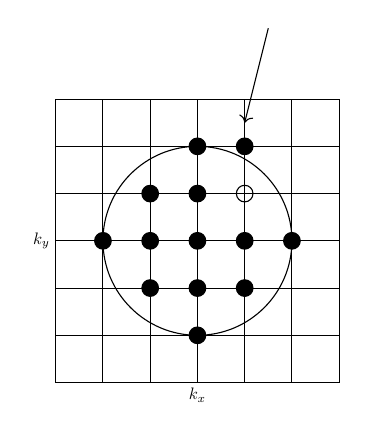
\begin{tikzpicture}[scale=0.6, transform shape]
			\draw(0,0)--(0,6)--(6,6)--(6,0)--(0,0);
			\draw(1,0)--(1,6);
			\draw(2,0)--(2,6);
			\draw(3,0)--(3,6);
			\draw(4,0)--(4,6);
			\draw(5,0)--(5,6);
			\draw (6,1)--(0,1);
			\draw (6,2)--(0,2);
			\draw (6,3)--(0,3);
			\draw (6,4)--(0,4);
			\draw (6,5)--(0,5);
			\filldraw[black] (3,3) circle (5pt);
			\filldraw[black] (4,3) circle (5pt);
			\filldraw[black] (2,3) circle (5pt);
			\filldraw[black] (3,2) circle (5pt);
			\filldraw[black] (3,4) circle (5pt);
			\filldraw[black] (5,3) circle (5pt);
			\filldraw[black] (1,3) circle (5pt);
			\filldraw[black] (3,1) circle (5pt);
			\filldraw[black] (3,5) circle (5pt);
			\draw[black] (4,4) circle (5pt);
			\filldraw[black] (2,2) circle (5pt);
			\filldraw[black] (2,4) circle (5pt);
			\filldraw[black] (4,2) circle (5pt);
			\draw(3,3) circle(2.0);
			\filldraw[black](4,5) circle(5pt);
			\draw[->](4.5,7.5)--(4,5.5);
			\node[anchor=east] at (0,3) {$k_y$};
			\node[anchor=north] at (3,0) {$k_x$};
		\end{tikzpicture}
	\end{subfigure}
	\hfill
	\begin{subfigure}[t]{0.45\textwidth}
		\caption{Energy required to move an electron from just below \gls{gls:fermi:surface} to above. We need a little bit of energy to move to the surface from below, plus a little to move to position above. We an think of the second as the energy of the electron, and the first as the energy of the hole. The electron might move around, and then suddenly pop into the hole, emitting a photon that takes away the extra energy. The hole is a fake particle with the opposite charge to an electron. It can come together with the electron and annihilate.}
		\begin{tikzpicture}[scale=0.6, transform shape]
			\draw (-5,0) to (5,0) node[anchor=east]{Fermi Surface};
			\filldraw[black] (3,2) circle (5pt);
			\draw(-1,-2) circle(5pt);
			\draw[->] (-1,-2) to (-1,-0.2);
			\draw[->] (-1,0) to (2.8,1.8);
		\end{tikzpicture}
	\end{subfigure}
\end{figure}

In Figure \ref{fig:fermions:move:ground:state} a charged hole is left behind.
If an electron drops into hole, a photon is emitted.

Consider an atom, with all electrons in their ground state. Low energy electron is struck by photon, which takes electron to excited state.

Electrons that are deep in \gls{gls:fermi:sea} can't be excited by low energy photons. Only shallow electrons are accessible.

\subsubsection{Dirac and antiparticles}

We start with the 1-dimensional case. Imagine a wave propagating to the right with speed $c$.
\begin{align*}
	\omega =& k\\
	\frac{\partial \psi}{\partial t} =& - \frac{\partial \psi}{\partial x}  \numberthis \label{eq:rh:dirac}\\
	\psi =& e^{i(kx-\omega t)} \numberthis \label{eq:rh:dirac:wave}
\end{align*}

What if $k$ negative? Then we have negative energy. But if we had arbitrarily negative energies, particle could keep emitting photons all the way down. So (\ref{eq:rh:dirac}) would not make sense for Fermions.

Dirac said to pretend that all the negative energy states were filled, just like filling the \gls{gls:fermi:sphere}: that is the lowest energy state, i.e. the \emph{vacuum}. Now we can take an electron out, leaving a hole. We then have two positive energy objects, electron and positron.( This only makes sense for Bosons, only Fermions). There are some things wrong with this electron:
\begin{itemize}
	\item it only moves to the right;
	\item it moves at the speed of light.
\end{itemize}

\section{The Dirac equation and the Higgs particles}

\subsection{The Dirac equation}

The simplest version of the Dirac Equation  (\ref{eq:rh:dirac}), applies to both electrons and positrons, provided they are moving to the right. We will start with the following equation:
\begin{align*}
	\Psi_R =& e^{i(kx-\omega t)} \text{The group velocity is:} \numberthis \label{eq:rh:dirac:wave1}\\
	V_g =& \frac{\omega}{k} \text{, assuming the relationship between $k$ and $\omega$ is linear.}
\end{align*}

If $V_g>0$ the wave moves to the right, otherwise it moves to the left.

Now, we write down another equation, c.f. \eqref{eq:rh:dirac}:
\begin{align*}
	\frac{\partial \Psi}{\partial t} + \frac{\partial \Psi}{\partial x} =&0 \text{. This has the solution \eqref{eq:rh:dirac:wave1}}, provided:\\
	\omega =& k
\end{align*}
If $k<0$, $\omega<0$, energy is negative, which is not a good thing: electrons would not be stable--Figure \ref{fig:negative:energy:rh}. So we fill up the \gls{gls:dirac:sea}, so all negative energy states are filled. Then we can remove one electron, creating a hole in the \gls{gls:dirac:sea}; particle and hole both have positive momentum (they move to the right) and positive energy.

\begin{figure}[H]
	\caption{Negative energy is not a good thing: electrons would not be stable}
	\begin{subfigure}[t]{0.45\textwidth}
		\caption{If $k<0$, $\omega<0$, energy is negative}\label{fig:negative:energy:rh}
		\begin{tikzpicture}[scale=0.45, transform shape]
			\draw(-5,0)--(5,0) node[right] {k};
			\draw(0,-5)--(0,5) node[above] {$\omega=E$};
			\draw(0,0)--(5,5) node[right] {$\omega=k$};
			\draw(2.5,2.5) node[midway] {$\\psi_R$};
			\draw[dashed,->](0,0)--(-4,-4) node[midway] {$E<0$};
			\draw(-4.5,-4.5) node {Electrons can slide down to $-\infty$};
		\end{tikzpicture}
	\end{subfigure}
	\hfill
	\begin{subfigure}[t]{0.45\textwidth}
		\caption{Add in left handed electrons.}\label{fig:negative:energy:lh}
		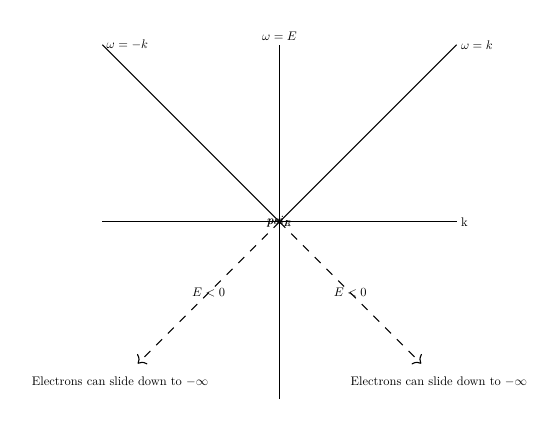
\begin{tikzpicture}[scale=0.45, transform shape]
			\draw(-5,0)--(5,0) node[right] {k};
			\draw(0,-5)--(0,5) node[above] {$\omega=E$};
			\draw(0,0)--(5,5) node[right] {$\omega=k$};
			\draw(2.5,2.5) node[midway] {$\\psi_R$};
			\draw(-2.5,2.5) node[midway] {$\\psi_L$};
			\draw[dashed,->](0,0)--(-4,-4) node[midway] {$E<0$};
			\draw(0,0)--(-5,5) node[right] {$\omega=-k$};
			\draw[dashed,->](0,0)--(4,-4) node[midway] {$E<0$};
			\draw(-4.5,-4.5) node {Electrons can slide down to $-\infty$};
			\draw(4.5,-4.5) node {Electrons can slide down to $-\infty$};
		\end{tikzpicture}
	\end{subfigure}
\end{figure}

We have strange situation: electrons that can only move to the right, plus an enormous negative momentum stored in the \gls{gls:dirac:sea}. What can we do to make it more symmetric? We now introduce two kinds of electrons, right movers and left movers.

\begin{align*}
	\frac{\partial \Psi_R}{\partial t} =& -\frac{\partial \Psi_R}{\partial x} \numberthis \label{eq:rh:dirac:wave:1}\\
	\frac{\partial \Psi_L}{\partial t} =& + \frac{\partial \Psi_L}{\partial x} \numberthis \label{eq:lh:dirac:wave}
\end{align*}

So, as shown in Figure \ref{fig:negative:energy:lh}, we have a bunch of particles with positive energy, and another with negative. How do we balance them? Fill sea with left moving negative energy. Then we have right moving particles, and holes, and left moving particles and holes. They are massless, because they move with the speed of light.

We will turn $\Psi_R$ and $\Psi_L$ into a columns vector. Define $\Psi=\begin{pmatrix}
	\Psi_R\\
	\Psi_L
\end{pmatrix}$, and write \eqref{eq:rh:dirac:wave:1} and \eqref{eq:lh:dirac:wave}:

\begin{align*}
	\frac{\partial \Psi}{\partial t} =& - \alpha \frac{\partial \Psi}{\partial x} \text{, where}\\
	\alpha =& \begin{pmatrix}
		1&0\\
		0&-1
	\end{pmatrix} \text{,or, in operator language:} \numberthis\label{eq:alpha}\\
	\omega =& \alpha k \numberthis \label{eq:dirac:1}
\end{align*}

We have turned two equations into one, but we haven't done any new physics. Can we make our massless particles have mass? Remember the relationship between mass and energy.

\begin{align*}
	\omega =& \sqrt{k^2 + m^2}  \numberthis \label{eq:omega:relativistic}
\end{align*}
If $m$ = 0, this is reminiscent of \eqref{eq:dirac:1}. We will generalize for $m\ne0$.
\begin{align*} 
	\omega =& \alpha k + m \beta  \numberthis \label{eq:Dirac:1D}
\end{align*}

This gives:
\begin{align*}
	\omega^2 =& \alpha^2 k^2 + m^2 \beta^2 + m k (\alpha \beta + \beta \alpha) \text{, which agrees with \eqref{eq:omega:relativistic} iff:}\\
	\alpha^2 =& 1 \text{, already satisfied by (\ref{eq:alpha})}\\
	\beta^2 =& 1 \text{, and}\numberthis \label{eq:beta2}\\ 
	\{\alpha,\beta\} =& 0 \numberthis \label{eq:alpha:beta}\\
	\beta =& \begin{pmatrix}
	0 & 1\\
	1 & 0
	\end{pmatrix} \text{ satisfies (\ref{eq:beta2}) and (\ref{eq:alpha:beta}).}
\end{align*}

The mass term couples equations for $\Psi_L$ and $\Psi_R$. The solution is Lorentz covariant.

\begin{align*}
	i \frac{\partial \Psi}{\partial t} =& -i \alpha \frac{\partial \Psi}{\partial x} + m \beta \Psi
\end{align*}
Let us go to the limit and make the particle stand still, i.e. $k=0 \implies \omega = \beta m$.

\begin{align*}
	i \frac{\partial \Psi}{\partial t} =& \beta m \Psi\\
	i \dot{\Psi_R} =& m \Psi_L\\
	i \dot{\Psi_L} =&  m \Psi_R \text{, now define}\\
	\Psi_+\triangleq&\Psi_R + \Psi_L \text{, and}\\
	\Psi_-\triangleq&\Psi_R - \Psi_L \text{, then} \\
	i \dot{\Psi_+} =&  m \Psi_+ \text{, corresponds to $\omega=m$}\\
	i \dot{\Psi_-} =&  -m \Psi_- \text{, corresponds to $\omega=-m$}
\end{align*}

So particle at rest still has positive and negative energies: throw latter in\gls{gls:dirac:sea}. The linear superposition $Psi_+$ corresponds to a particle with positive energy at rest.

What is the meaning of operators such as $\Psi_+$? What is the effect of $\Psi_+\ket{0}$? A single particle, which has equal probability of being a left mover or a right mover. In general a particle is a superposition of a left and a right mover.

\subsection{Higgs particles}

What is the connection between the notion of mass, as introduced above, and the notion that the Higgs field produces mass? In the presence of the Higgs field, $\Phi(x)$, the Dirac equation becomes:
\begin{align*}
	i \dot{\Psi_R} =& -i \partial_x \Psi_R + g \Phi \Psi_L\\
	i \dot{\Psi_L} =& i \partial_x \Psi_L + g \Phi \Psi_R
\end{align*}
If $\Phi=0$ we once again have a massless electron. What if the lowest energy of Higgs favours a non-zero value, $\Phi(x)=\phi$? See Figure \ref{fig:higgs:potential}. Then $m=g\phi$. That is the connection. It could come about as the result of non-linear interactions between Boson and Fermions.

The Higgs field is a Bosonic field, which has an energy from a potential, $V(\phi)$.  It differs from the Maxwell field, whose potential that depends on gradients of the field. There is a symmetry so $V(\phi)=V(-\phi)$.

The Higgs field can vibrate, as shown in Figure \ref{fig:vibrating:higgs:field}: the frequency is related to the mass of the Higgs particle, and the excitation, like that of any field, come in quanta. Those quanta are the Higgs particle.
\begin{figure}[H]
	\caption[The Higgs potential]{The Higgs potential: the reason for its shape was not fully understood at time of the lecture.}
	\begin{subfigure}[t]{0.3\textwidth}
		\begin{center}
			\caption{The Higgs potential, showing two minima, at $\pm\phi$. Either one gives rise to mass of $g\phi$. If there were only one minimum we could take it to be zero, and it would not give rise to a mass term.}\label{fig:higgs:potential}
			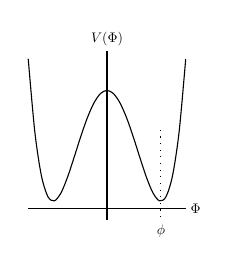
\begin{tikzpicture}[scale=0.5, transform shape]
				\draw(-2,-2)--(2,-2) node[right] {$\Phi$};
				\draw(0,-2.3)--(0,2) node[above] {$V(\Phi)$};
				\draw[domain=-2:2, smooth, variable=\x, ] plot ({\x}, {1-3*\x*\x+0.8*\x*\x*\x*\x});
				\draw[dotted](1.3693,0)--(1.3693,-2.3) node[below] {$\phi$};
			\end{tikzpicture}
		\end{center}
	\end{subfigure}
	\hfill
	\begin{subfigure}[t]{0.3\textwidth}
		\begin{center}
			\caption{The Higgs field vibrating around vacuum. The frequency is related to the mass of the Higgs particle: the Higgs corresponds to quanta of vibration.}\label{fig:vibrating:higgs:field}
			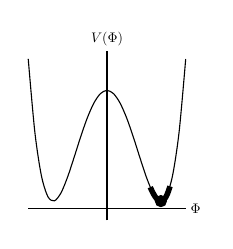
\begin{tikzpicture}[scale=0.5, transform shape]
				\draw(-2,-2)--(2,-2) node[right] {$\Phi$};
				\draw(0,-2.3)--(0,2) node[above] {$V(\Phi)$};
				\draw[domain=-2:2, smooth, variable=\x, ] plot ({\x}, {1-3*\x*\x+0.8*\x*\x*\x*\x});
				\draw[domain=1.1:1.6,  line width=2pt, smooth, variable=\x, ] plot ({\x}, {1-3*\x*\x+0.8*\x*\x*\x*\x});
				\filldraw[black] (1.3693,-1.8125) circle (4pt);
			\end{tikzpicture}
		\end{center}
	\end{subfigure}
	\hfill
	\begin{subfigure}[t]{0.3\textwidth}
		\begin{center}
			\caption{The Higgs field vibrating around vacuum with enough energy to make electron massless; this energy is enormous, enough to create a black hole.}\label{fig:vibrating:higgs:field:massless:electron}
			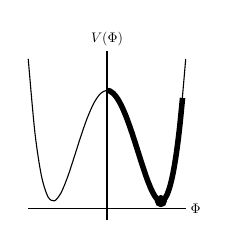
\begin{tikzpicture}[scale=0.5, transform shape]
				\draw(-2,-2)--(2,-2) node[right] {$\Phi$};
				\draw(0,-2.3)--(0,2) node[above] {$V(\Phi)$};
				\draw[domain=-2:2, smooth, variable=\x, ] plot ({\x}, {1-3*\x*\x+0.8*\x*\x*\x*\x});
				\draw[domain=0:1.92,  line width=2pt, smooth, variable=\x, ] plot ({\x}, {1-3*\x*\x+0.8*\x*\x*\x*\x});
				\filldraw[black] (1.3693,-1.8125) circle (4pt);
			\end{tikzpicture}
		\end{center}
	\end{subfigure}
\end{figure}

If the Higgs field is coupled in an interesting dynamical way to Fermions, the Higgs field will respond to collisions of Fermions by vibrating, and create Higgs particles. How much energy is needed? It depends on the mass of the Higgs particle. The vibration of the Higgs field can affect the mass of the electron--Fugure \ref{fig:vibrating:higgs:field:massless:electron}.

In the Standard Model there is only one Higgs particle, one for all Fermions, Supersymmetry has two.

If vacuum were symmetric--Figure \ref{fig:higgs:potential}-- $\phi$ would be zero: it is the breaking of the symmetry which gives electron its mass. All particles, except the photon and graviton\footnote{They aren't really exceptions: they have \emph{no} mass.}, get their mass through the Higgs Mechanism. Except for Higgs particle: it gets its mass from a totally different mechanism.

\subsection{The 3+1 Dimensional Dirac Equation}

Particles are described by a frequency, and a wave vector, which replaces the wave number. The wave vector is proportional to the momentum. Dirac began by writing down a generalization of a generalization of \eqref{eq:Dirac:1D}:

\begin{align*}
	\omega =& \alpha . k+\beta m\\
	=& \alpha_1 k_1 + \alpha_2 k_2 + \alpha_3 k_3 +\beta m \numberthis \label{eq:omega:3D}
\end{align*}

Given that $\vec{k}$ has 3 components, $\alpha$ needs 3 also. In 3 dimensions, \eqref{eq:omega:relativistic} generalizes to:
\begin{align*}
	\omega^2 =& k_1^2 + k_2^2 +k_3^2 +m^2 \text{, but \eqref{eq:omega:3D} gives}\\
	=& (\alpha_1 k_1 + \alpha_2 k_2 + \alpha_3 k_3 +\beta m)(\alpha_1 k_1 + \alpha_2 k_2 + \alpha_3 k_3 +\beta m)
\end{align*}
These expressions agree iff:
\begin{align*}
	\alpha_i^2 =& 1  \text{ and} \numberthis \label{eq:dirac:ac1}\\
	\beta^2 =& 1 \text{ and} \numberthis \label{eq:dirac:ac2}\\
	\{\alpha_i,\alpha_j\} =& 2 \delta_{i,j} \numberthis \label{eq:dirac:ac3}\\
	\{\alpha_i,\beta\} =& 0 \numberthis \label{eq:dirac:ac4}
\end{align*}

Theorem \ref{thm:dirac:anticommutation} shows 2 or 3 dimensional matrices cannot satisfy these equations; $4 \times 4$ is the first case.

Here is a set of Dirac Matrices (not unique, but equivalent--Theorem \ref{thm:dirac:anticommutation} presents a different set).

\begin{align*}
	\beta =& \begin{pmatrix}
		1&0&0&0\\
		0&1&0&0\\
		0&0&-1&0\\
		0&0&0&-1
	\end{pmatrix} \numberthis \label{eq:beta:1}\\
	\alpha_1 =& \begin{pmatrix}
		0&0&0&1\\
		0&0&1&0\\
		0&1&0&0\\
		1&0&0&0
	\end{pmatrix}\numberthis \label{eq:alpha1:1}\\ 
	\alpha_2 =& \begin{pmatrix}
		0&0&0&-i\\
		0&0&i&0\\
		0&-i&0&0\\
		i&0&0&0
	\end{pmatrix} \numberthis \label{eq:alpha2:1} \\ 
	\alpha_3 =& \begin{pmatrix}
		0&0&1&0\\
		0&0&0&-1\\
		1&0&0&0\\
		0&-1&0&0 
	\end{pmatrix} \numberthis \label{eq:alpha3:1}
\end{align*}

A simpler notation is to divide into blocks of $2\times 2$ matrices, and use the Pauli matrices (\ref{eq:pauli:x}), (\ref{eq:pauli:y}), and (\ref{eq:pauli:z}):
\begin{align*}
	\beta = \begin{pmatrix}
		I&0\\
		0&I
	\end{pmatrix} \numberthis \label{eq:dirac:block:1}\\
	\alpha = \begin{pmatrix}
		0&\sigma\\
		-\sigma&0
	\end{pmatrix} \numberthis \label{eq:dirac:block:2}
\end{align*}

\begin{align*}
	\psi =& \begin{pmatrix}
		\psi_1\\
		\psi_2\\
		\psi_3\\
		\psi_4
	\end{pmatrix} \text{ spinor--left/right and spin up/down}\\
	i \frac{\partial \psi}{\partial t} =& -i \alpha_i \frac{\partial \psi}{\partial x^i} + \beta m \psi \text{, the famous Dirac equation} \numberthis \label{eq:famous:dirac}
\end{align*}

Although $\Psi$ has 4 components, it is \emph{not} a 4-vector.

\section{Angular momentum}

Our goal is to understand an important idea, \emph{spin}.

Angular momentum is a vector, which points along the axis of rotation and follows the right hand rule: fingers follow rotation, thumb points along vector.

An object has two kinds of angular momentum:
\begin{itemize}
	\item orbital angular momentum--motion of centre of mass relative to an axis, even if the object is not itself spinning about an internal axis;
	\item spin angular momentum, the kind we are interested in, is the angular momentum in a frame where the centre of mass is at rest.
\end{itemize}

If we start a basketball rotating, it remains the same basketball. In \glsdesc{gls:QM} the amount of angular momentum is discrete, which can't interpolate between different amounts of angular momentum; is it the same object at each level? How much energy does it take to set it into rotation? Whether it is the same object or not is a matter of definition.

Is a rotating nucleus the same object as a non-rotating nucleus? Note that angular momentum is quantized, so it takes a discrete amount of energy to start rotation. Now an atom with too much rotation will fly apart, which is definitely different. 

What about electron? Is it too small for us to rotate? Does it make sense to talk about a point-like object rotating?  Maybe it isn't infinitely small? The smaller the object, the more energy it needs to rotate with a given amount of angular momentum. Maybe the electron is too small.

The angular momentum for a small object like an electron \emph{characterizes} the object, and it is fixed.

Let us invent a particle with definite angular momentum, a ''spintron''. Can it point in any direction? Yes, since the laws of physics are rotationally invariant. But the amount of angular momentum is quantized.

The theory is mathematical: it seems abstract, but corresponds to experiment.

Classically we have the  moment of inertia, which depends on the  mass, and how it is distributed. The only thing new in \glsdesc{gls:QM} is the quantization of $L$.
\begin{align*}
	I\triangleq&mr^2 \\
	L\triangleq&mVr\text{, we can show}\\
	E=&\frac{L^2}{2I}\\
	=&\frac{L^2}{2mr^2}\\
	I\rightarrow&0 \text{ as $r \rightarrow 0 $, whence } \\
	\rightarrow &\infty \text{ as } r \rightarrow 0 \text{ for discrete $L$}
\end{align*}

Let us consider a single particle orbiting a centre--Figure \ref{fig:one:particle:rotating}. The Angular momentum is $pr$. it has angular momentum because it has momentum, and it has momentum because it has velocity. This is not spin.

Figure \ref{fig:two:particles:rotating} depicts two particles rotating: the centre of mass is at rest, so the total momentum is zero, but there is angular momentum. This \emph{is} spin.

\begin{figure}[H]
	\caption{Angular momentum for rotating particles}
	\begin{subfigure}[t]{0.45\textwidth}
		\caption{A single particle rotating about a centre. The system has angular momentum $L=pr$, because it has momentum.}\label{fig:one:particle:rotating}
		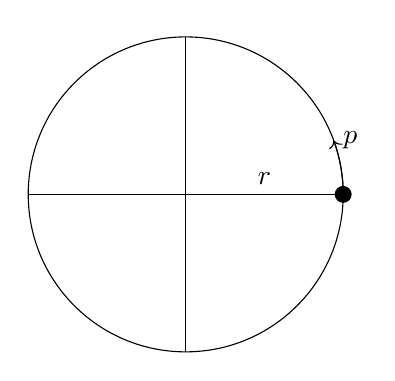
\begin{tikzpicture}
			\draw(-2,0)--(2,0) node[right] {};
			\draw(0,-2)--(0,2) node[right] {};
			\draw (0,0) circle (2);
			\filldraw (2,0) circle (0.1);
			\draw[->] (2,0) arc [radius=2,start angle=0, end angle=20] node[right] {$p$};
			\draw(1,0) node[above] {$r$};
		\end{tikzpicture}
	\end{subfigure}
	\hfill
	\begin{subfigure}[t]{0.45\textwidth}
		\caption{Two particles rotating. the centre of mass is at rest, so the total momentum is zero, but there is angular momentum. This \emph{is} spin}\label{fig:two:particles:rotating}
		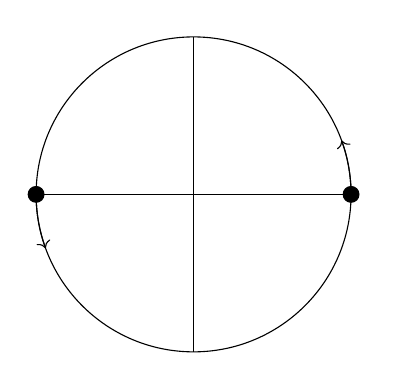
\begin{tikzpicture}
			\draw(-2,0)--(2,0) node[right] {};
			\draw(0,-2)--(0,2) node[right] {};
			\draw (0,0) circle (2);
			\filldraw (2,0) circle (0.1);
			\filldraw (-2,0) circle (0.1);
			\draw[->] (2,0) arc [radius=2,start angle=0, end angle=20] ;
			\draw[->] (-2,0) arc [radius=2,start angle=180, end angle=200];
		\end{tikzpicture}
	\end{subfigure}
\end{figure}

Classically, and in \glsdesc{gls:QM}, the orbital angular momentum of a point particle moving about origin is given by:
\begin{align*}
	\vec{L} =& \vec{R} \times \vec{p} \\
	L_x =& y P_z - z P_y\\
	L_y =& z P_x - x P_z\\
	L_z =& x P_y - y P_x
\end{align*}

Moving to \glsdesc{gls:QM}, we will determine commutation relations of angular momentum operators. Once we have them we can forget the definitions of the $Lx$.The commutators are all we need to work out everything else.

\begin{thm}[Commutators for angular momentum]
	\begin{align*}
	[L_x,L_y]=& i \hslash L_z \numberthis \label{eq:lx:ly}\\
	[L_y,L_x]=& i \hslash L_x \numberthis \label{eq:ly:lz}\\
	[L_z,L_x]=& i \hslash L_y \numberthis \label{eq:lz:lx}	
	\end{align*}
\end{thm}
\begin{proof}
	We have, from \cite{susskind2014quantum}:
	\begin{align*}
		[X_i,X_j] =& 0\\
		[P_i,P_j]=& 0\\
		[X_i,P_j]=& i \hslash \delta_{i,j}
	\end{align*}

	\begin{align*}
			[L_x,L_y]=& [y P_z - z P_y,z P_x - x P_z]\\
	=&[y P_z, z P_x] -\cancel{[yP_z,xP_z]} -\bcancel{[zP_y,zP_x]} + [z P_y,x P_z]
	\end{align*}
	Where we have used $[yP_z,xP_z]=xy[P_z,P_z]=0$.
	\begin{align*}
		[L_x,L_y]=& y P_x[P_z,z] + P_y x[z,P_z]\\
		=& -i \hslash y P_x + i \hslash P_y x\\
		=& i \hslash L_z \text{, which is (\ref{eq:lx:ly})} 
	\end{align*}
	The other two equations, (\ref{eq:ly:lz}) and (\ref{eq:lz:lx}) follow by cyclically permuting indices.
\end{proof}

 These relationships:
\begin{itemize}
	\item remain true if we add angular momenta for many particles;
	\item are true for spin;
	\item are rotationally invariant;
	\item explain why $\hslash$ appears in the quantum of angular momentum.
\end{itemize}

We focus on the $z$-axis, which we call the ''quantization access''. There is nothing special about $z$; we could have used $x$ or $y$ and developed the same theory. We introduce two new  operators, which will turn out to be raising and lowering operators, analogous to those for the Harmonic Oscillator. Choosing units where $\hslash=1$:

\begin{align*}
	L_\pm \triangleq& L_x \pm i L_y \numberthis \label{eq:L_pm} \\
\end{align*}
We'll calculate some commutators:
\begin{align*}
	[L_+,L_z] =& [L_x+i L_y,L_z]\\
	=& -iL_y + i^2 L_x \text{, from (\ref{eq:lz:lx}) and (\ref{eq:lx:ly})}\\
	=& -L_+ \text{ from (\ref{eq:L_pm}).} \numberthis \label{eq:L+:Lz}\\
\end{align*}
Similarly
\begin{align*}
	[L_-,L_z]  =& [L_x-i L_y,L_z]\\
	=&-iL_y - i^2 L_x\\
	=& L_x-iL_y\\
	=& L_- \numberthis \label{eq:L-:Lz}
\end{align*}

\begin{thm}[$L_+$ is a creation operator for $L_z$] \label{thm:angular:momentum:creation}
	\begin{align*}
		L_z \ket{m} =& m \ket{m} \numberthis \label{eq:L:eigen}\\
		\implies&\\
		L_z (L_+ \ket{m}) =& (m+1) L_+ \ket{m}
	\end{align*}	
\end{thm}

\begin{proof}
	We use 	\eqref{eq:L+:Lz}
	\begin{align*}
		L_+L_z-L_zL_+ =& -L_+ \text{, whence:}\\
		L_zL_+ =& L_+L_z + L_+\ \text{ and}\\
		L_z L_+ \ket{m} =& (L_+L_z + L_+)\ket{m}\\
		=& L_+ (L_z + I)\ket{m}\\
		=& L_+ (m + 1) \ket{m} \text{ from (\ref{eq:L:eigen})}\\
		=&  (m + 1) L_+ \ket{m}
	\end{align*}
\end{proof}

\begin{cor}[$L_-$ is an annihilation  operator for $L_z$]\label{thm:angular:momentum:annihilation}
	\begin{align*}
	L_z \ket{m} =& m \ket{m} \\
	\implies&\\
	L_z (L_- \ket{m}) =& (m-1) L_- \ket{m}
	\end{align*}	
\end{cor}
\begin{proof}
	We use \eqref{eq:L-:Lz}
	\begin{align*}
		L_-L_z - L_zL_-=&L_- \\
		L_zL_- =& L_-L_z - L_- \\
		L_zL_-\ket{m} =& L_-L_z\ket{m} - L_-\ket{m}\\
		=& m L_-\ket{m} - L_-\ket{m}\\
		 =& (m-1) L_- \ket{m}
	\end{align*}
\end{proof}
The angular momentum spectrum is spaced by integers. Can it go on forever? How far can we bump $L_z$ up before the object changes? Imagine a classical object with fixed $L^2$. We can maximize $L_z$  by pointing it upward.

Theorem \ref{thm:angular:momentum:creation} and Corollary \ref{thm:angular:momentum:annihilation} ignore the possibility that $L^+m_{max}=0$ and $L^-m_{min}=0$. (c.f. harmonic oscillator). By rotational invariance, $m_{min}=-m_{max}$: spectrum must be symmetric about zero.

There are two possibilities for the spectrum:
\begin{itemize}
	\item $-m_{max},...,-1,0,1,...m_{max}$
	\item $-m_{max},...,-\frac{1}{2},\frac{1}{2},...m_{max}$
\end{itemize}

\begin{defn}[Spin]
	$m_{max}$ is known as the spin. It can be 0. There are no elementary particles known with spin 3, but there are nuclei. Similarly no half-spin particle over $\frac{3}{2}$.
\end{defn}

What about $L^2$? If you know $L_z$ at maximum, there will be uncertainty in other two components, so $L^2$ is not quite $m_{max}^2$.

\begin{align*}
	L_- L_+ =& (L_x-iL_y)(L_x+iL_y)\\
	=& L_x^2 +i L_x L_y -i L_y L_x + L_y^2\\
	=& L_x^2 + L_y^2 + i[L_x,L_y]\\
	=& L^2 - L_z^2 + i[L_x,L_y] \numberthis \label{eq:L-:L+}
\end{align*}

Hence, classically:
\begin{align*}
	L^2 =& L_- L_+ + L_z^2
\end{align*}

This is not true for quantum world! Instead \eqref{eq:L-:L+} implies:
\begin{align*}
	 L^2 =& L_- L_+ + L_z^2 -\underbrace{i[L_x,L_y]}_\text{$i^2L_z$ from (\ref{eq:lx:ly})}\text{, in the quantum world}\\
	=& L_- L_+ + L_z^2 +L_z\\
	L^2 \ket{m_{max}}=& L_- L_+ \ket{m_{max}} + L_z^2 \ket{m_{max}} +L_z \ket{m_{max}}\\
	=& (0 +m_{max}^2 + m_{max})\ket{m_{max}} \\
	=& m_{max} (m_{max}+1)\ket{m_{max}}
\end{align*}
All states have same value of $\braket{L^2}$. 

\begin{thm}[$L^2$ commutes with all its components.]
	 \begin{align*}
	 [L^2,L_i]=0  \;\forall i \in {x,y,z}
	 \end{align*}
\end{thm}
\begin{proof}
	We need the following lemma.
	\begin{lemma}[Commutator with square]\label{lemma:comm:sq}
		\begin{align*}
			[A^2,B] =& A[A,B] + [A,B]A
		\end{align*}
	\end{lemma}
	\begin{proof}[Proof of lemma]
		\begin{align*}
			[A^2,B] =& AAB - BAA\\
			=& AAB - ABA +ABA -BAA\\
			=& A[A,B] + [A,B]A
		\end{align*}
	\end{proof}
	\begin{align*}
	[L^2,L_x]=&[L_x^2,L_x] + [L_y^2,L_x] + [L_z^2,L_x] \numberthis \label{eq:L2lx}\\
	[L_y^2,L_x] =&L_y[L_y,L_x] + [L_y,L_x]L_y \text{, using Lemma \ref{lemma:comm:sq}}\\
	=& -i L_y L_z -i L_z L_y \text{ from (\ref{eq:ly:lz}). Similarly}\\
	[L_z^2,L_x] = &L_z [L_z,L_x] + [L_z,L_x] L_z\\
	=& i L_z L_y  + i L_y L_z \text{ from (\ref{eq:lz:lx}), whence (\ref{eq:L2lx}) yields}\\
	[L^2,L_x]=&\cancel{[L_x^2,L_x] }+\bcancel{ [L_y^2,L_x]} + \bcancel{[L_z^2,L_x]}\\
	=& 0
	\end{align*}
\end{proof}
Consider spin $\frac{1}{2}$--call them $\ket{+}$ and  $\ket{-}$.

\begin{align*}
	e^{i\theta} \alpha \ket{+} + e^{i\theta}\beta \ket{-} \text{, has probability $\alpha^2$ of being in $\ket{+}$}
\end{align*}
So can ignore 1 degree of freedom. The parameters $\alpha$ and $\beta$ have 2 degrees of freedom each. Phase eliminates one, and $\alpha^2+\beta^2=1$ eliminates one other, leaving two. This is the same as number of degrees of freedom in direction.

The measured value is always $\pm \frac{1}{2}$; average may be zero; it behaves like a classical variable.

\begin{thm}[Spin statistics]
	\begin{enumerate}
		\item All particles with half integral spin are Fermions;
		\item All particles with  integral spin are Bosons.
	\end{enumerate}
\end{thm}

\begin{proof}
	TBP
\end{proof}
Take two half spin particles: composite behaves like a Boson--e.g. Hydrogen atom; deuteron is Boson, deuterium is Fermion.


\section{Spin}

\subsection{Combining Fermions to make Bosons}

Paradox: if two Fermions make a Boson, can we have two of these composite Bosons in the same state?

Wave function of Bosons is supposed to be symmetric under interchange of two Bosons. Consider two Bosons, at positions $x$ and $y$. Since there is no difference between them:

\begin{align*}
	\psi(x,y) =&\psi(y,x) \text{, e.g. a product}\\
	\psi(x,y) =& \phi(x)\phi(y) \text{, which would correspond to two Bosons $\phi$}\\
	\phi(x)\phi(y) =& \phi(y)\phi(x) \text{, wave functions aren't operators--they commute.}
\end{align*}
So we could have two Bosons in exactly the same state.

The rule for Fermions is:
\begin{align*}
		\psi(x,y) =&-\psi(y,x)
\end{align*}

So we can't have two of them in the same state.

Now imagine a wave function, $\psi(x,y)$, that isn't symmetric or antisymmetric. We construct symmetric and antisymmetric functions.
\begin{align*}
	\psi(x,y)+& \psi(y,x) \text{ symmetric--a possible wave function for Bosons}\\
	\psi(x,y)-& \psi(y,x) \text{ antisymmetric--a possible wave function for Fermions}
\end{align*}

Now imagine four Fermions: two electrons, which we will call $x$, and two protons, which we will call $y$. Our wave function is a function of four variables: $\psi(x_1,x_2,y_1,y_2)$.

\begin{align*}
	\psi(x_1,x_2,y_1,y_2) = &-\psi(x_2,x_1,y_1,y_2) \text{, electrons are Fermions}\\
	=& - \psi(x_1,x_2,y_2,y_1) \text{, protons are Fermions}
\end{align*} 

Imagine a hydrogen atom at the origin, $\psi(x_1,y_1)$ plus another hydrogen atom, $\phi(x_2,y_2)$, so the wavefunction for the system is $\psi(x_1,y_1)\phi(x_2,y_2)$. This isn't symmetric for the $x$s or the $y$s, so it isn't a good wavefunction for Fermions. Suppose we make it antisymmetric:
\begin{align*}
	\psi(x_1,y_1) \phi(x_2,y_2) -& \psi(x_2,y_1) \phi(x_1,y_2) 
	-\psi(x_1,y_2) \phi(x_2,y_1) + \psi(x_2,y_2) \phi(x_1,y_1)\\
	x_1 \leftrightarrow& x_2 \text{ interchange electrons--changes sign, and}\\
	y_1 \leftrightarrow& y_2 \text{ interchange protons--changes sign, but}\\
	1 \leftrightarrow& 2 \text { interchange atoms--preserves sign.}
\end{align*}

What if both atoms have same wave function? Ignoring a factor of $2$:

\begin{align*}
	\psi(x_1,y_1) \psi(x_2,y_2) -& \psi(x_2,y_1) \psi(x_1,y_2) 
\end{align*}

Both atoms can be in same place, although it costs a lot of energy, but we can't find 2 electrons in same place. In an atom the electron does not have a well defined position, 

\subsection{The Mathematics of Spin}

The mathematics of Spin is needed for the study of Isospin, Colour, etc. We will start with half spin, and will call our particles ''electrons''. They could easily be muons, quarks, etc. 

\subsubsection{Half spin}

We will call these particles ''electrons'', even though they might be muons, quarks, or whatever.

We have two values along the z axis: $S_z = m \hslash$, although we will set $\hbar=1$ from now on (This is not the full angular momentum). We will use $S$ for spin, $L$ for orbital angular momentum. The mathematics of $S$ is the same as that of $L$--see \eqref{eq:lx:ly},  \eqref{eq:ly:lz}, and  \eqref{eq:lz:lx}.

\begin{align*}
	[S_x,S_y] =& i S_z \numberthis \label{eq:sx:sy}\\
	[S_y,S_z] =& i S_x  \numberthis \label{eq:sy:sz}\\
	[S_z,S_x] =& i S_y \text{, and we define the raising and lowering operators} \numberthis \label{eq:sz:sx}\\
	S_\pm \triangleq& S_x \pm S_y 
\end{align*}

For the time being, we forget everything about the electron, except for spin, so we have a space of two orthogonal states, which we can write as a column vector:
\begin{align*}
	\begin{pmatrix}
		\alpha\\
		\beta
	\end{pmatrix} \text{, or}\\
	\psi = \alpha\ket{+} + \beta\ket{-}
\end{align*}


The operators are $2\times 2$ matrices satisfying algebra \eqref{eq:sx:sy}, \eqref{eq:sy:sz}, and \eqref{eq:sz:sx}. They are not unique, but all representations are equivalent. We will use the Pauli spin matrices\footnote{Without $\frac{1}{2}$ they are known as Pauli matrices.}:
\begin{align*}
	S_x =& \frac{1}{2}\begin{pmatrix} \numberthis \label{eq:pauli:x}
		0&1\\
		1&0
	\end{pmatrix}\\
	S_y =& \frac{1}{2}\begin{pmatrix} \numberthis \label{eq:pauli:y}
		0&-i\\
		i&0
	\end{pmatrix}\\
	S_z =& \frac{1}{2}\begin{pmatrix} \numberthis \label{eq:pauli:z}
		1&0\\
		0&-1
	\end{pmatrix}
\end{align*}

[I have omitted the discussion of eigenvectors of the $S_i$].

\subsubsection{Spin 1}

We have  a Boson with three spin states $\{-1,0,1\}$. Are there $3\times3$ matrices satisfying \eqref{eq:sx:sy}, \eqref{eq:sy:sz}, and \eqref{eq:sz:sx}? Yes: they aren't unique, and here is one such set.

\begin{align*}
	S_z = i \begin{pmatrix}
		0&1&0\\
		-1&0&0\\
		0&0&0
	\end{pmatrix}\\
	S_y = i \begin{pmatrix}
		0&0&1\\
		0&0&0\\
		-1&0&0
	\end{pmatrix}\\
	S_x = i \begin{pmatrix}
		0&0&0\\
		0&0&1\\
		0&-1&0
	\end{pmatrix}
\end{align*}

Find eigenstates of $S_z$:
\begin{align*}
	i \begin{pmatrix}
		0&1&0\\
		-1&0&0\\
		0&0&0
	\end{pmatrix}\begin{pmatrix}
		\alpha\\
		\beta\\
		\gamma
	\end{pmatrix}=&\begin{pmatrix}
		\alpha\\
		\beta\\
		\gamma
	\end{pmatrix}\\
	=&i\begin{pmatrix}
		\beta\\
		-\alpha\\
		0
	\end{pmatrix}
\end{align*}
So the eigenvectors are:
\begin{align*}
	\frac{1}{\sqrt(2)}\begin{pmatrix}
		1\\
		-i\\
		0
	\end{pmatrix}\\
	\frac{1}{\sqrt(2)}\begin{pmatrix}
		1\\
		i\\
		0
	\end{pmatrix}\\
	\begin{pmatrix}
		0\\
		0\\
		1
	\end{pmatrix}\\
\end{align*}
Suppose that we return to real electron, which can move in space. It has a position (or momentum) and spin. How does we represent it with a position, given that it has spin and position? We turn the 2D spinor components into functions of position: if the electron is found at $x$, what is the probability that it is up?
\begin{align*}
	&\begin{pmatrix}
		\psi_u(x)\\
		\psi_d(x)
	\end{pmatrix} \text{, and or spin 1:}\\
	&\begin{pmatrix}
		\phi_1(x)\\
		\phi_2(x)\\
		\phi_3(x)
	\end{pmatrix}
\end{align*}


\subsection{Dirac Equation: connection with Spin}

The Dirac equation was given in \eqref{eq:famous:dirac}:
\begin{align*}
	i \frac{\partial \psi}{\partial t} =& - i \alpha_i \frac{\partial \psi}{\partial x^i} + \beta m \psi\\
	\omega =& \sum_i \alpha_i k_i + \beta m\\
	\omega^2 =& k^2 + m^2
\end{align*}
Where the $\alpha_i$ and $\beta$ satisfy \eqref{eq:dirac:ac1}, \eqref{eq:dirac:ac2}, \eqref{eq:dirac:ac3}, and \eqref{eq:dirac:ac4}.

\begin{thm}[Dirac anticommutation relations.]\label{thm:dirac:anticommutation} 
	\begin{enumerate}
		\item Equations \eqref{eq:dirac:ac1}, \eqref{eq:dirac:ac2}, \eqref{eq:dirac:ac3}, and \eqref{eq:dirac:ac4} can be satisfied by suitably chosen $4\times4$ matrices\label{eq:step1};
		\item  they cannot be satisfied by $2 \times 2$ matrices or $3 \times 3$ matrices\label{eq:step2}.
	\end{enumerate}
\end{thm}
\begin{proof}
	 Part \ref{eq:step1}: we exhibit a set of solutions in \eqref{eq:dirac:block:1} and \eqref{eq:dirac:block:2}.
	 
	 Part \ref{eq:step2} TBP.
\end{proof}

One set of solutions, which is not the same as \eqref{eq:dirac:block:1} and \eqref{eq:dirac:block:2}:
\begin{align*}
	\alpha_i=&\begin{pmatrix}
		\sigma_i&0\\
		0&-\sigma_i
	\end{pmatrix}\\
	\beta =& \begin{pmatrix}
		0&I\\
		I&0
	\end{pmatrix}
\end{align*}

The difference between \eqref{eq:dirac:block:1} and \eqref{eq:dirac:block:2} and this set is a rotation in the 4 dimensional representational space: the 4 components are not a relativistic 4-vector!

There are two kinds of $2\times2$ness, which corresponds to a doubling in the physics: one kind is to do with the fact that there are two energies, positive and negative, the other is spin. There are particles with positive energy and all sorts of spins, particles with nagative energy and all sorts of spins.
The 4 components are not a relativistic 4-vector! The easiest way to see this is to set momentum to zero, then the $\alpha_i$ drop out.

For a particle at rest.

\begin{align*}
	i \frac{\partial \psi}{\partial t} =&  \beta m \psi \text{. We decompose $\psi$ into 2 2 component objects.}\\
	i \frac{\partial}{\partial t}\begin{pmatrix}
		\psi_+\\
		\psi_-
	\end{pmatrix}=&m \begin{pmatrix}
		0&I\\
		I&0
	\end{pmatrix}\begin{pmatrix}
		\psi_+\\
		\psi_-
	\end{pmatrix} \text{, we get a pair of coupled equations}\\
	i \frac{\partial \psi_+}{\partial t} =&   m \psi_-\\
	i \frac{\partial \psi_-}{\partial t} =&   m \psi_+ \text{. Introduce new variables to uncouple.}\\
	i \frac{\partial (\psi_++\psi_-)}{\partial t} =&   m (\psi_++\psi_-) \text{ Energy $\omega=m>0$}\\
	i \frac{\partial (\psi_+-\psi_-)}{\partial t} =&   -m (\psi_+-\psi_-) \text{ Energy, $\omega=-m<0$}
\end{align*}

So as with \eqref{eq:rh:dirac:wave:1} and \eqref{eq:lh:dirac:wave} we have positive and negative energy solutions, each of which is a 2 dimensional entity, which is spin. How do we see that this is really spin? We want to see that a positive energy pair is spin, we need to look at angular momentum. We can look at the connection between angular momentum and rotation symmetry, or at conservation of momentum.

We want to show that in any form of collision, where an electron scatters of something else, that if you assign the electron an angular momentum whose description is in terms of the 2-foldness of $\sigma$, that total angular momentum would be conserved.

\section{Equations of motion of particles and fields}\label{sect:equation:motion}

A very important concept in particle physics are the field equations, the equations of motion of fields that describe particles, boson fields, fermionic fields, the electromagnetic fields. All these fields satisfy equations. These are more or less wave equations, which involve derivatives with respect to space and to time, and the field itself. How do we code these equations? They all come from a Lagrangian, which contains, in one compact expression, all the fields in a system, and all the degrees of freedom.

\subsection{Review of classical fields}

The Lagrangian of a system of fields

\begin{align*}
	\mathcal{L}=& \mathcal{L}(\phi,\partial_t \phi, \partial_x \phi)\\
	=&\mathcal{L}(\phi,\partial_{\mu} \phi) \text{ in Minkowski space}
\end{align*}

The equations of motion are:
\begin{align*}
	\frac{\partial}{\partial t} \frac{\partial \mathcal{L}}{\partial \big(\frac{\partial \phi}{\partial t}\big)}+\sum_i \frac{\partial}{\partial x_i} \frac{\partial \mathcal{L}}{\partial \big(\frac{\partial \phi}{\partial x_i}\big)}=&\frac{\partial \mathcal{L}}{\partial \phi} \numberthis \label{eq:lagrange}
\end{align*}

(If $\mathcal{L}$ depends on several fields, there will be a version of (\ref{eq:lagrange})  for each field.)

Example of $\mathcal{L}$.

\begin{align*}
	\mathcal{L} =& \frac{1}{2} (\frac{\partial \phi}{\partial t})^2 - \frac{1}{2} (\frac{\partial \phi}{\partial x})^2 - \frac{1}{2} (\frac{\partial \phi}{\partial y})^2 - \frac{1}{2} (\frac{\partial \phi}{\partial z})^2 - V(\phi)
\end{align*}

Substituting in (\ref{eq:lagrange}):
\begin{align*}
	\ddot{\phi} - \frac{\partial^2 \phi}{\partial x^2}  - \frac{\partial^2 \phi}{\partial y^2}  - \frac{\partial^2 \phi}{\partial z^2} =& - \frac{\partial V}{\partial \phi}
\end{align*}

$V(\phi)$ is field energy. If it is not bounded below, the minimum is infinitely far away, which isn't good.  The simplest interesting case is:
\begin{align*}
	V(\phi) =& \frac{m^2 \phi^2}{2}\\
	\ddot{\phi} - \frac{\partial^2 \phi}{\partial x^2}  - \frac{\partial^2 \phi}{\partial y^2}  - \frac{\partial^2 \phi}{\partial z^2} =& - m^2 \phi \numberthis \label{eq:simplest:non:trivial}
\end{align*}

This is a wave equation. What does it say about the relationship between energy and momentum of a quantum of the field? Differentiating a wave function $e^{-i \omega t} e^{-i k x}$ twice by $t$ gives a factor $-\omega^2$. Substituting in (\ref{eq:simplest:non:trivial}):
\begin{align*}
	-\omega^2 \phi - (k_x^2+k_y^2+k_z^2)\phi =& -m^2 \phi \text{, or, canceling}\\
	-\omega^2  - (k_x^2+k_y^2+k_z^2) =& -m^2 \\
	E^2 + P^2 = m^2 \text{, the usual relation in relativity}
\end{align*}

If $\mathcal{L}$ is a scalar, the equations of momentum will be Lorentz Invariant.

What about a more complex $V(\phi)$?
\begin{align*}
	V(\phi) =& \frac{m^2 \phi^2}{2} + g \phi^3\\
	\ddot{\phi} - \frac{\partial^2 \phi}{\partial x^2}  =& - m^2 \phi - 3 g \phi^2
\end{align*}

Quadratic terms in Lagrangian lead to linear equations; different solution pass right through each other, even though they may interfere. Higher powers lead to non-linearities, so we cannot superpose solutions. The wave packets scatter.

Consider two scalar fields:
\begin{align*}
	\mathcal{L} =& \frac{1}{2}(\partial_{\mu} \phi)^2 + \frac{1}{2}(\partial_{\mu} \rho)^2 - \frac{m^2 \phi^2}{2} - \frac{M^2 \rho^2}{2} - \rho \phi^2
\end{align*}
The equations of motions are:
\begin{align*}
	\ddot{\phi} - \partial_x^2 \phi =& -m^2 \phi - \rho \phi\\
	\ddot{\rho} - \partial_x^2 \rho =& -M^2 \rho -\phi^2
\end{align*}

These are non-linear and coupled, so the particles scatter each other. Terms like $\rho \phi^2$ are telling us something about the interaction.

Consider the Dirac equation.

\begin{align*}
	\dot{\psi} =& i \alpha \frac{\partial \psi}{\partial x} + m \beta \psi \text{, which can be generated by the Lagrangian}\\
	\mathcal{L} =& i \big( \psi^\dagger \partial_t \psi +  \psi^\dagger \alpha \partial_x \psi + \psi^\dagger \beta \psi m \big)
\end{align*}

Suppose there is another field: we can add a scalar field to Dirac field and get scattering, and generate equations of motion for both fields.

\begin{align*}
	\mathcal{L} =& i \big( \psi^\dagger \partial_t \psi +  \psi^\dagger \alpha \partial_x \psi + \psi^\dagger \beta \psi m \big) +...- \psi^\dagger \beta \psi \phi
\end{align*}

The Lagrangian is what specifies a field theory.

\subsection{Quantum Fields}

\subsubsection{The Lagrangian codifies the interaction in the system.}

We have already talked about the scattering of particles, and how it represented by products of fields. Fields are built up out of creation and annihilation operators. Let us start with a field  $\phi^3$, what does that represent in terms of creation and annihilation operators?The field will contain both creation and annihilation operators, $\phi = (a_+ + a_-)$, and, when it is cubed, we will have all sorts of terms, which can annihilate 3 particles, etc. So $\phi^3$ has a meaning in terms of particles coming in and particles going out.

Imagine Lagrangian containing $\phi^3$, where $\phi = (a_+ + a_-)$.
Figure \ref{fig:phi:3:x} shows the kinds of interaction that may occur.
 
\begin{figure}[H]
	\caption{$\phi^3(x)$ gives rise to many possible interactions.}\label{fig:phi:3:x}
	\begin{subfigure}[t]{0.2\textwidth}
		\caption{One particle going in, two going out}
		\feynmandiagram[scale=0.5,transform shape][vertical = out1 to in1]{
			in1--[fermion]c[particle=\(x\)],
			c--[fermion]out1,
			c--[fermion]out2,
		};
	\end{subfigure}
	\hfill
	\begin{subfigure}[t]{0.2\textwidth}
		\caption{Two particles going in, one out}
		\feynmandiagram[scale=0.5,transform shape][vertical = out2 to c]{
			in1--[fermion]c[particle=\(x\)],
			in2--[fermion]c,
			c--[fermion]out2,
			in1--[opacity=0.0]in2
		};
	\end{subfigure}
	\hfill
	\begin{subfigure}[t]{0.2\textwidth}
		\caption{Three particles going out from nothing}
		\feynmandiagram[scale=0.5,transform shape][vertical = out1 to c]{
		c[particle=\(x\)]--[fermion]out1,
		c--[fermion]out2,
		c--[fermion]out3,
		out1--[opacity=0.0]out2,
		out1--[opacity=0.0]out3
	};
	\end{subfigure}
	\hfill
	\begin{subfigure}[t]{0.2\textwidth}
		\caption{Three particles going in, nothing coming out}
		\feynmandiagram[scale=0.5,transform shape][vertical = c to in1]{
			in1--[fermion]c[particle=\(x\)],
			in2--[fermion]c,
			in3--[fermion]c,
			in1--[opacity=0.0]in2,
			in1--[opacity=0.0]in3
		};
	\end{subfigure}
\end{figure}
Quadratic terms in Lagrangian give rise to motion, higher powers to interactions. Let us see how the quadratic terms work.

How to change the position of a particle? We need a pair of operators $\phi(x) \phi(x^\prime)$ to absorb particle at $x$, and re-emit at $x^\prime$--i.e. move particle.

\begin{align*}
	\frac{1}{2}(\frac{\partial \phi}{\partial x})^2 =& \frac{1}{2}\frac{\big( \phi(x) - \phi(x^\prime)\big)^2}{...}\\
	=& \frac{\frac{1}{2}\phi(x)^2 + \frac{1}{2}\phi(x^\prime)^2 -  \phi(x) \phi(x^\prime)}{...}
\end{align*}

The first two terms on the right hand side are not very interesting: they remove a particle at a point, and put it back again. $\phi(x) \phi(x^\prime)$ absorbs a particle at one point and puts it back somewhere else: it \emph{moves} the particle. Quadratic terms move the undisturbed particle: they are connected with free motion. Higher powers bring particles together, to create and annihilate them.

The Lagrangian codifies the interaction in the system.

\begin{figure}[H]
	\begin{center}
		\caption[The mass term $m^2\phi^2$]{The mass term $m^2\phi^2$ absorbs particle and re=emits it from the same point: in effect it \emph{counts} particles.}
		\feynmandiagram[vertical = out1 to in1]{
			in1--[fermion]c[particle=\(x\)],
			c--[fermion]out1
		};
	\end{center}
\end{figure}

\subsubsection{Electromagnetic field and Dirac electron.}

This is the basic process of \glsdesc{gls:QED}, which is a description of electrons and photons. Electrons are described by the Dirac field. $\Psi$ is built up from annihilation operators:
\begin{align*}
	\Psi =& c_e^-(\text{+ve energy}) + c_e^-(\text{-ve energy})\\
	\Psi^\dagger =& c_e^+(\text{+ve energy}) + c_e^+(\text{-ve energy}
\end{align*}
Now an annihilation operator for a particle of negative energy can be relabeled as a creation operator for an antiparticle of positive energy (since a positron is a hole in the Dirac Sea).

\begin{align*}
	\Psi =& c_e^-(\text{+ve energy}) + c_p^+(\text{+ve energy}) \\
	\Psi^\dagger =&  c_e^+(\text{+ve energy}) + c_p^-(\text{+ve energy})
\end{align*}

Now the basic interaction of electrodynamics is:
\begin{align*}
	e \big( \Psi^\dagger \Psi A_0 + 	\Psi^\dagger \alpha_i  \Psi A_i \big)  \numberthis \label{eq:basic:interaction}
\end{align*}
Where $A$ is the field operator for photons. Photons have a directionality, their polarization. We take the inner product of $A$ and the 4-vector $(\Psi^\dagger \Psi, \Psi^\dagger \alpha_i  \Psi) $ to make a scalar. $A$ contains creation and annihilation operators for photons.

\begin{figure}[H]
	\caption{Examples of interactions arising from Lagrangian--Equation \eqref{eq:basic:interaction}}\label{fig:psi:dagger:psi:A}
	\begin{subfigure}[t]{0.3\textwidth}
		\begin{center}
			\caption{Annihilation + 2 creation: photon emitted}
			\feynmandiagram[scale=0.5,transform shape][vertical = out1 to in1]{
			in1[particle=\(e\)]--[fermion]c,
			c--[fermion]out1,
			c--[photon]out2,
			out1--[opacity=0.0]out2
			};
		\end{center}
	\end{subfigure}
	\hfill
	\begin{subfigure}[t]{0.3\textwidth}
		\begin{center}
			\caption{2 Annihilation +  creation: photon absorbed}
			\feynmandiagram[scale=0.5,transform shape][vertical = out1 to in1]{
				in1[particle=\(e\)]--[fermion]c,
				c--[fermion]out1,
				in2--[photon]c,
				in1--[opacity=0.0]in2
			};
		\end{center}
	\end{subfigure}
	\hfill
	\begin{subfigure}[t]{0.3\textwidth}
		\begin{center}
			\caption{2 Annihilation +  creation: Electron + positron produce photon.}
			\feynmandiagram[scale=0.5,transform shape][vertical = out1 to c]{
				in1[particle=\(e^-\)]--[fermion]c,
				in2[particle=\(e^+\)]--[anti fermion]c,
				c--[photon]out1,
				in1--[opacity=0.0]in2,
			};
		\end{center}
	\end{subfigure}
	\begin{subfigure}{0.3\textwidth}
		\begin{center}
			\caption{Photon absorbed, electron and positron created.}
			\feynmandiagram[scale=0.5,transform shape][vertical = out1 to c]{
				in1--[photon]c,
				c--[fermion]out1[particle=\(e^-\)],
				c--[anti fermion]out2[particle=\(e^+\)],
				out1--[opacity=0.0]out2,
			};
		\end{center}
	\end{subfigure}
	\hfill
	\begin{subfigure}{0.3\textwidth}
		\begin{center}
			\caption{Photon, electron and positron absorbed (energy and momentum not conserved!).}\label{fig:em:dirac5}
			\feynmandiagram[scale=0.5,transform shape][vertical =c to in2]{
				in1[particle=\(e^-\)]--[fermion]c,
				in2[particle=\(e^+\)]--[anti fermion]c,
				in3--[photon]c,
				in1--[opacity=0.0]in2,
				in2--[opacity=0.0]in3,
			};
		\end{center}
	\end{subfigure}
\end{figure}

The processes depicted in Figure \ref{fig:psi:dagger:psi:A} are all produced by $ \Psi^\dagger \Psi A$, and they all have the same numerical coefficient:
$e$, the electric charge of the electron, is the strength of interaction; the probability of interaction is $e^2$ (Consider an electron hitting a wall: $e$ is the dimensionless probability that it emits a photon).

Remember that energy conservation arose from integrating over all time, and momentum conservation from integrating over space. If we integrate \eqref{eq:basic:interaction} over all space and all time,  energy and momentum will both be conserved, which rules out the process depicted in Figure \ref{fig:em:dirac5}. So once we have drawn Figure \ref{fig:psi:dagger:psi:A} and worked out the amplitudes, we still need to integrate over all time and space to ensure that energy and momentum will be conserved.

\subsubsection{Protons, Neutrons, and Pi mesons}.

Protons, neutrons, and pi mesons form a system that is similar to \glsdesc{gls:QED} in spirit. Protons and neutrons are Fermions. Pions are scalar particles, and they come in 3 varieties, $\pi_+$, $\pi_-$, and $\pi_0$.

\begin{table}[H]
	\begin{center}
		\caption{Protons, Neutrons, Pi mesons}
		\begin{tabular}{|l|l|} \hline
			Operators &Description\\ \hline
			$\Psi_p$, $\Psi^\dagger_p$& create and annihilate proton\\ \hline
		    $\Psi_n$, $\Psi^\dagger_n$& create and annihilate neutron\\ \hline
			$\pi_+$& annihilate pion\\ \hline
			$\pi_-$&annihilate pion\\ \hline
			$\pi_0$&annihilate pion\\ \hline
			$\Psi^\dagger_p \Psi_n \pi_+$&Absorb pion and neutron, emit proton\\ \hline
			$\Psi^\dagger_n \Psi_p \pi_-$&Absorb pion and proton, emit neutron\\ \hline
			$\Psi^\dagger_p \Psi_p \pi_0$&Absorb pion and proton, emit proton\\ \hline
			$\Psi^\dagger_n \Psi_n \pi_0$&Absorb pion and neutron, emit neutron \\ \hline
		\end{tabular}
	\end{center}
\end{table}
These aren't really fundamental processes; the real thing involve quarks, but the description with proton, neutron and mesons fields worked when we didn't know about quarks, or when energies are low enough. If the energy is high enough to break up protons, we cannot use proton fields.

\begin{figure}[H]
	\caption{The same interaction can describe several processes: $\Psi^\dagger_n \pi^\dagger_+ \Psi_n$}
	\begin{subfigure}[p]{0.45\textwidth}
		\begin{center}
			\caption{Proton $\rightarrow$ neutron + pion}
			\feynmandiagram[vertical =out1 to in1]{
				in1[particle=\(p\)]--[fermion]c,
				c--[fermion]out1[particle=\(n\)],
				c--[boson]out2[particle=\(\pi^+\)],
				out1--[opacity=0.0]out2
			};
		\end{center}
	\end{subfigure}
	\hfill
	\begin{subfigure}[p]{0.45\textwidth}
		\begin{center}
			\caption{Proton + antineutron $\rightarrow$ pion}
			\feynmandiagram[vertical =out1 to in1]{
				in1[particle=\(p\)]--[fermion]c,
				in2[particle=\(\bar{n}\)]--[anti fermion]c,
				c--[boson]out1[particle=\(\pi^+\)],
				in1--[opacity=0.1]in2
			};
		\end{center}
	\end{subfigure}
\end{figure}

The Lagrangian describes things that happen at a point, or a pair of neighbouring points. Figure \ref{fig:proton:electron:photon} shows an interaction arising from a product of terms. There is no action at a distance in \glsdesc{gls:QFT}.
\begin{figure}[H]
	\begin{center}
		\caption[Proton photon electron interaction]{Proton photon electron interaction--product of two separate terms in Lagrangian. The interaction between the proton and the photon, and the electron and the photon, occur at two separate points: the proton needs to be moved from one point to the other by a quadratic term, which builds up (e.g.) $xy$ out of infinitesimal moves.}\label{fig:proton:electron:photon}
		\feynmandiagram[vertical = out1 to in1]{
			in1[particle=\(e\)]--[fermion]c1[particle=y]--[fermion]out1[particle=\(e\)],
			in2[particle=\(p\)]--[fermion]c2[particle=x]--[fermion]out2[particle=\(p\)],
			c1--[photon]c2,
			in1--[opacity=0]in2
		};
	\end{center}
\end{figure}
 
In  Figure \ref{fig:proton:electron:photon} we have a process taking place at $x$, another at $y$, plus a vast number moving the photon along the line joining them (derivative terms). There is no term in the Lagrangian describing Figure \ref{fig:proton:electron:photon}. It is built up from a large number of basic units; you have to compound them together to make the general process. The Lagrangian is make up out of fields, which are made up out of creation and annihilation operators; it can occur at many places, and we multiply these  instance. The Lagrangian is not something which is a final answer; it describes the basic elements which compound themselves by product.

A single field can absorb \emph{or} spit out a particle; a product of two fields can absorb \emph{and} spit out a particle.

The Heisenberg uncertainty principle says that we either describe things in terms of position or momentum, not both. The creation operators and annihilation operators are functions of either position or momentum, never both. The creation operator $\Psi(x)=\sum_{p}a_pe^{ipx}$. We never have $\Psi(p,x)$, i.e. we never create at bth $p$ and $x$. The Fourier transform is the essence of the uncertainty principle.
NB: creation operators are functions of P or X, never both (). They are related through Fourier transforms, which are the essence of the uncertainty principle.

An experiment looks like this: $\bra{0}\psi^\dagger\psi^\dagger\psi^\dagger...\mathcal{L}\mathcal{L}\mathcal{L}...\psi\psi\psi\ket{0}$. We start with the vacuum, do stuff with Lagrangians, then detect the results. The interactions are coded in simple form in the Lagrangian. This makes it easy to deal with symmetries. For example, in \eqref{eq:basic:interaction}, we can multiply $\Psi$ by $e^{i\theta}$, $\Psi^\dagger$ by $e^{-i\theta}$, and the Lagrangian remains unchanged: this is a statement of charge conservation, equal numbers of $\Psi$  and  $\Psi^\dagger$. We multiply lots of Lagrangians.

There was a question about eigenvalues and eigenvectors of the field operators. The eigenvectors of the electromagnetic field are measurable. Now creation and annihilation operators don't commute, so field operators don't commute. Now $[\Phi(x),\Phi(y)]\ne 0$ for $x\ne y$: you can not simultaneously measure the field operator at two different positions.

Can we simplify the product of Lagrangians?

\begin{align*}
	\Pi_i& \big(1+\mathcal{L}_{interaction}(x_i)\big)\\
	=&1 + \sum_i \underbrace{ \mathcal{L}(x_i)}_\text{one vertex}  +\sum_{i,j}\underbrace{\mathcal{L}(x_i)\mathcal{L}(x_j)}_\text{two vertices} +...
\end{align*}

We get an infinite number of places where 1 thing, 2 things, etc, happen.

The art form is figuring out the Lagrangian from experimental data; then \glsdesc{gls:QFT} becomes a precise tool.

Often we can ignore parts of Lagrangian: e.g. quarks don't have much to do with electrons, so we can ignore them in \glsdesc{gls:QED}. LS suggested that \glsdesc{gls:QFT} may be a coarse grained description of something else.
 

\section{Field Lagrangians and Path Integrals}

The basic technique that Lecture \ref{sect:equation:motion} alluded to is called the \emph{path integral method of quantum mechanics}. It is the most direct route to the theory of particle interactions based on Feynman diagrams. The path integral is the quantum mechanical version of the Principle of Least Action\cite{susskind2013quantum}. If we think of a classical Newtonian particle, its motion from one point of space-time to another is determined by a Lagrangian $\mathcal{L}(\dot{X},X)$. We use the Lagrangian to construct the Action. 

\begin{defn}[Classical Action of Path]
	For every trajectory, $P$ from the initial point to the final point, whether or not the trajectory is a solution to Newton's Laws of motion,  the Classical Action is: 
	\begin{align*}
		\mathcal{A}=\int_P dt \mathcal{L}(\dot{X},X)
	\end{align*}
\end{defn}


The classical form of the Principle of Least Action is that the true trajectory minimizes the action. We can use the calculus of variations to derive differential equations which satisfy Newton's Laws. The same idea works in classical field theory, where $\mathcal{L}=\mathcal{L}(\phi,\partial_\mu\phi)$. The theory of relativity requires that the Lagrangian be a scalar\cite{susskind2017special}.

\begin{defn}[Action over Region]
	For a region of spaces time, $R$,  the Action is: 
	\begin{align*}
		\mathcal{A}=\int_R dx^4 \mathcal{L}(\phi,\partial_\mu\phi)
	\end{align*}
\end{defn}

The analogue of the starting point for a particle is the initial value of the field. If we prescribe the starting and final values of the field, we can ask whether there is a solution that starts with starting values, and ask whether there is a solution that minimizes the action. The principle of least action states that the correct value of the field is the one that minimizes the action. So the original principal of least action gets extended to a space-time principal of least action, where the degrees of freedom are fields. NB, we are looking for a way to interpolate the field which minimizes the Action.
\url{https://youtu.be/q-QaaKCvDUs?t=555}
We now look at the quantum mechanical use of Action: \emph{we won't attempt to derive the classical version from the quantum mechanical version.}

According to quantum mechanics, a thing that you might want to calculate is the \emph{amplitude}, so we can calculate probabilities. Imagine that particle is injected at $(x,t)$: what is amplitude that particle will be found at $(x^\prime,t^\prime)$?

Feynman's rule is:

\begin{align*}
	Amplitude =& \sum_{Histories} e^{-\frac{i}{\hslash} \int \mathcal{L} dt}
\end{align*}

where the sum is taken over all classically \emph{possible} histories--Figure \ref{fig:sum:histories}--i.e. they can not go back in time for non-relativistic QM. Probability is the square of the magnitude of the Amplitude.

\begin{figure}[H]
	\caption{Sum over histories}\label{fig:sum:histories}
	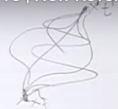
\includegraphics[width=0.8\textwidth]{sum-histories}
\end{figure}



Imagine starting systems with field $\phi(x)$, and asking for probability of $\phi^\prime(x)$ at some later time--Figure \ref{fig:path-integral1}. Again this is determined by an amplitude:
\begin{align*}
	\sum e^{-\frac{i}{\hslash} \int dx dy dz dt\mathcal{L}(\phi,\partial \phi) }
\end{align*}
summed over all possible histories between $\phi(x)$ and $\phi^\prime(x)$.

\begin{figure}[H]
	\caption{Initial and final conditions}\label{fig:path-integral1}
	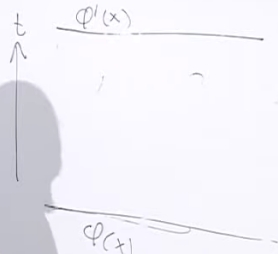
\includegraphics[width=0.8\textwidth]{path-integral1}
\end{figure}

(A question was asked about convergence: trajectories tend to cancel, and those with the least cancellation tend to be near the ones that have least action classically.)

There are two ways to think of quantum field theory, in terms of fields, and in terms of particles. What if we specify field quanta (particles)? We ask the probability of some specified particle content at a later time. The answer involves a path integral. Start by partitioning space into cells--Figure \ref{fig:path-integral2}--and think about the value of the field in each cell. We compute:
\begin{align*}
	\Pi_{i\in cells}(1-\frac{i}{\hslash} \mathcal{L_i}a^4) \text{, where $a^4$ is volume of a cell.}
\end{align*}
 
Now we have the following approximation for small $\epsilon$
\begin{align*}
	1 + \epsilon \approx &e^\epsilon\\
	\approx& 1 + \frac{\epsilon}{1!} + \frac{\epsilon^2}{2!}  + \frac{\epsilon^3}{3!} +...\\
\end{align*}

\begin{align*}
	\sum_{histories} e^{-\frac{i}{\hslash} \int dx dy dz dt\mathcal{L}(\phi,\partial \phi) } =& \sum_{histories} e^{-\frac{i}{\hslash} A_i } \text{, where $A_i$ is action in $i$th cell}\\
	=& \sum_{histories} \Pi_i e^{-\frac{i}{\hslash} A_i }
\end{align*}

Let's forget particles for a moment and think of fields.

\begin{figure}[H]
	\caption[Space partitioned into cells]{Space partitioned into cells. Initial conditions in bottom row, final in top. We consider all possible histories that match initial and final conditions. NB: functions aren't necessarily analytic or even continuous.}\label{fig:path-integral2}
	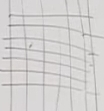
\includegraphics[width=0.8\textwidth]{path-integral2}
\end{figure}

Our question is now: if initial condition matches our initial configuration of particles, and final condition matches desired configuration, what is the amplitude? Figure \ref{fig:path-integral3} depicts a particle moving in one history.

\begin{figure}[H]
	\caption[Particle moving]{Creation operator in one cell, annihilation in neighbour amounts to movement}\label{fig:path-integral3}
	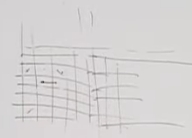
\includegraphics[width=0.8\textwidth]{path-integral3}
\end{figure}

There are terms in the Lagrangian associated with pairs of boxes--the derivatives:
\begin{align*}
	\frac{1}{2}(\partial_t \phi)^2 \rightarrow& \frac{1}{2}\frac{(\phi(t,x)-\phi(t^\prime,x))^2}{...}\\
	\frac{1}{2}(\partial_x \phi)^2 \rightarrow& \frac{1}{2}\frac{(\phi(t,x)-\phi(t,x^\prime))^2}{...} \numberthis \label{eq:phi:phi}
\end{align*}
(\ref{eq:phi:phi}) gives rise to terms such as:
\begin{alignat*}{2}
	e^{- i \sum_{neighbours} \phi(x) \phi(x^\prime)}=1& -&& i \sum_{neighbours} \underbrace{\phi(x) \phi(x^\prime)}_\text{Figure \ref{fig:path-integral5}}\\
	&-&& \frac{1}{2!}\underbrace{\sum_{neighbours} \phi(x) \phi(x^\prime)\sum_{neighbours} \phi(x^{\prime\prime}) \phi(x^{\prime\prime\prime})}_\text{Figure \ref{fig:path-integral7}}\\
	&+&&\underbrace{i\frac{1}{3!}\sum_{neighbours}\phi(..)\phi(..)\sum_{neighbours}\phi(..)\phi(..)\sum_{neighbours}\phi(..)\phi(..)}_\text{Figure \ref{fig:path-integral9}}\\
	&+&& ... \numberthis \label{eq:path:integral:expanded}
\end{alignat*}



\begin{figure}[H]
	\caption{Rules for Path Integrals}
	\begin{subfigure}{0.45\textwidth}
		\caption{Create at one point, annihilate at neighbour}\label{fig:path-integral5}
		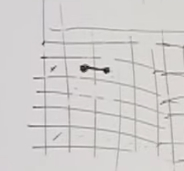
\includegraphics[width=1.0\textwidth]{path-integral5}
	\end{subfigure}
	\begin{subfigure}{0.45\textwidth}
		\caption{A dangling endpoint is illegal unless one endpoint creates, other annihilates: since we are only putting particles in from initial state and removing from final, this is illegal.}\label{fig:path-integral4}
		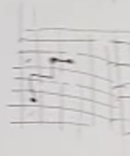
\includegraphics[width=1.0\textwidth]{path-integral4}
	\end{subfigure}
	\begin{subfigure}{0.45\textwidth}
		\caption{The only way Figure \ref{fig:path-integral5} can contribute is if space is only two layers thick.}\label{fig:path-integral6}
		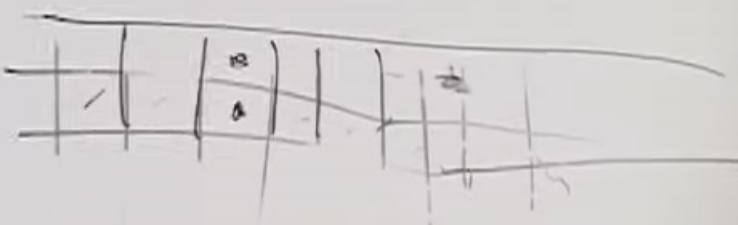
\includegraphics[width=1.0\textwidth]{path-integral6}
	\end{subfigure}
	\begin{subfigure}{0.45\textwidth}
		\caption{What about thicker space? How to we get from \ref{fig:path-integral6} to here? We need the quadratic term in (\ref{eq:path:integral:expanded})}\label{fig:path-integral7}
		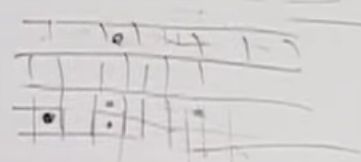
\includegraphics[width=1.0\textwidth]{path-integral7}
	\end{subfigure}
	\begin{subfigure}{0.45\textwidth}
		\caption{How to avoid dangling ends in \ref{fig:path-integral7}? Restrict to 3 layers. This allows us to find $x^\prime=x^{\prime\prime}$ in (\ref{eq:path:integral:expanded})}\label{fig:path-integral8}
		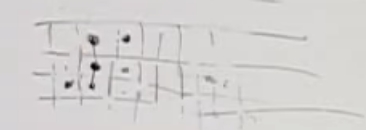
\includegraphics[width=1.0\textwidth]{path-integral8}
	\end{subfigure}
	\begin{subfigure}{0.45\textwidth}
		\caption{Including the cubic term in (\ref{eq:path:integral:expanded}) allows us to find two 3-step paths in (\ref{eq:path:integral:expanded}).}\label{fig:path-integral9}
		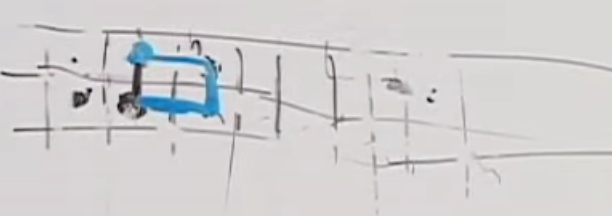
\includegraphics[width=1.0\textwidth]{path-integral9}
	\end{subfigure}
\end{figure}

So we can sum up contributions $\frac{i^n}{n !}$ in (\ref{eq:path:integral:expanded}) to determine complex amplitude. We include backward paths from special relativity--Figure \ref{fig:path:backward:time}.

\begin{figure}[H]
	\caption{Path going backwards in Time. We can think of it in two ways.}\label{fig:path:backward:time}
	\begin{subfigure}{0.45\textwidth}
		\caption{New rule allows particle to go back in time}
		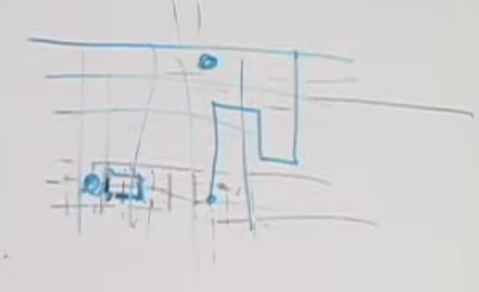
\includegraphics[width=0.8\textwidth]{path-backward-time}
	\end{subfigure}
	\begin{subfigure}{0.45\textwidth}
		\caption{Particle anti-particle pair used instead.}
		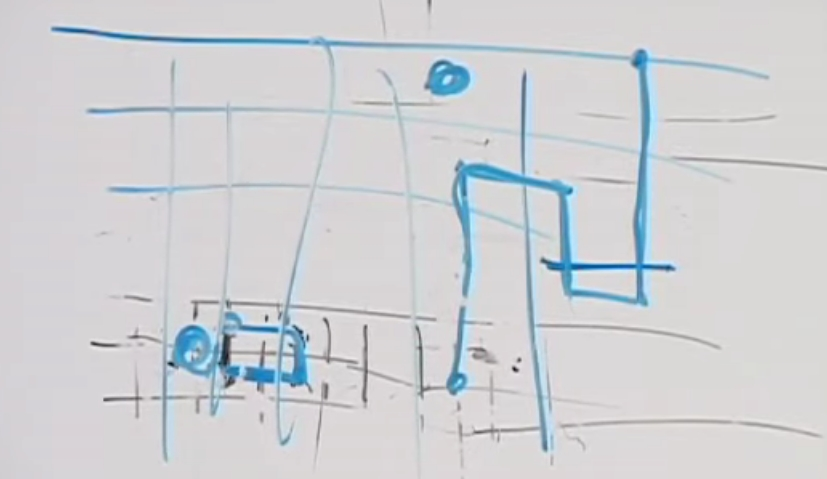
\includegraphics[width=0.8\textwidth]{path-backward-time1}
	\end{subfigure}
\end{figure}

Two particles.

\begin{figure}[H]
	\caption{Two particles}\label{fig:path:integral:2particles:1}
	\begin{subfigure}{0.45\textwidth}
		\caption{Quadratic term in (\ref{eq:path:integral:expanded}) used to advance two particles by one box}
		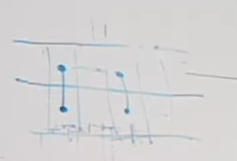
\includegraphics[width=0.8\textwidth]{path-integral-2particles-1}
	\end{subfigure}
	\begin{subfigure}{0.45\textwidth}
		\caption{Weight particle by $m^2$ from $\frac{m}{2}\phi^2$}\label{fig:path:integral:mass}
		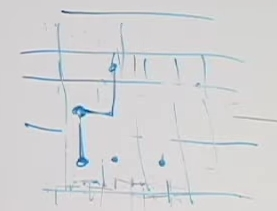
\includegraphics[width=0.8\textwidth]{path-integral-mass}
	\end{subfigure}
\end{figure}

What goes in Lagrangian?

\begin{align*}
\mathcal{L}=& \frac{1}{2} (\partial_t \phi)^2 - \frac{1}{2} (\partial_x \phi)^2 + \underbrace{\frac{m}{2}\phi^2}_\text{ absorb and emit at same point} +\underbrace{g \phi^3}_\text{Figure \ref{fig:path:integral:cubic}}
\end{align*}

This weights path by $m^2$--Figure \ref{fig:path:integral:mass}. If not used we have theory of massless particles.

\begin{figure}[H]
	\caption{Some possibilities from $\phi^3$}
	\begin{subfigure}{0.4\textwidth}
	\caption{Particle absorbed and two new particles created.}\label{fig:path:integral:cubic}
		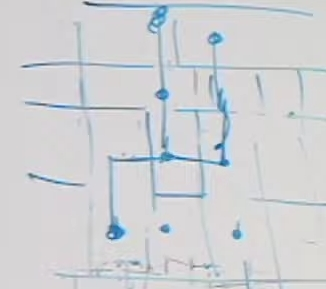
\includegraphics[width=0.8\textwidth]{path-integral-cubic}
	\end{subfigure}
	\begin{subfigure}{0.4\textwidth}
		\caption{Particle emitted and later reabsorbed.}\label{fig:path:integral:cubic:split}
		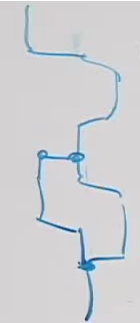
\includegraphics[width=0.8\textwidth]{path-integral-cubic-split}
	\end{subfigure}
	\begin{subfigure}[t]{0.4\textwidth}
		\begin{center}
			\caption{Electron emits and absorbs photon.}\label{fig:path:integral:cubic:split1}
			\feynmandiagram[vertical = out1 to in1]{
				in1--[fermion]a--[fermion]b--[fermion]out1,
				a--[photon,half right]b,
			};
		\end{center}
	\end{subfigure}
	\hfill
	\begin{subfigure}[t]{0.4\textwidth}
		\caption{More complex version of Figure \ref{fig:path:integral:cubic:split1}.}\label{fig:path:integral:cubic:split2}
		\feynmandiagram[vertical = d to a]{
			in1--[fermion]a--[fermion]b--[fermion]c--[fermion]d--[fermion]out1,
			b--[photon,half right]c,
			a--[photon]e--[fermion,quarter right]f0--[fermion,quarter right]f1--[photon]d,
			e--[anti fermion,quarter left,looseness=2]e1--[anti fermion,quarter left,looseness=2]f1,
			f0--[photon]e1,
		};
	\end{subfigure}
\end{figure}

How come answer not infinite? Powers of coefficients from Lagrangian $(g)$ appear with different powers; hope they are small enough.

Feynman diagrams and Lagrangians are complementary.

% glossary: may need command makeglossaries particles1
\printglossaries

\bibliographystyle{unsrt}
\addcontentsline{toc}{section}{Bibliography}
\bibliography{tm}

\end{document}
